\chapter{Detector commissioning}
\label{ch:commissioning}

The commissioning of the SuperNEMO demonstrator has begun in $2019$ and first calorimeter data was taken.\\
The calorimeter of SuperNEMO is segmented in $712$ optical modules (OM), each composed by a coupling between a photomultiplier tube (PMT) and a polystyrene scintillator bloc (see Sec.~\ref{sec:calorimeter} for more details).
The divider of a PMT is connected to $2$ cables, one providing the high voltage (HV), the other one, called signal cable, is a coaxial cable collecting and transporting the charge provided by the PMT.\\
By the summer $2020$, the SuperNEMO demonstrator will be encapsulated in an anti radon tent.
The so called \emph{patch panel} will insure passage of cables from the inside, to the outside of the anti radon tent, therefore doubling the amount of cables needed for the calorimeter.
We refer to the cables running from detector to patch panel as \emph{internal} cables, and the cables from patch panel to the electronic boards as \emph{external} cables.
Consequently, regarding only the calorimeter part, 2848 cables were cut, assembled, connector-mounted, transported and installed at LSM.
Then the check of every cable condition is mandatory to control and eventually fix them.

\section{Reflectometry analysis}
\label{sec:reflecto}

\subsection{Goal of the reflectometry analysis}

Taking into account the final demonstrator design, each coaxial length was determined, cables were cut and labelled in LAL, Orsay.
All external coaxial cables were designed to be $7$ meters-long -- the distance between electronic boards and patch panel being the same for all channels at electronic boards -- and internal cable lengths have been adapted to fit the distance from the patch panel to each optical module.
Then, cutting and labelling all cables lasted several weeks.
After all cables were transported and installed at LSM, we had to check each coaxial cable condition, for several reasons:
\begin{itemize*}
\item check if no cable was damaged during the transport and the installation;
\item control if no swap between cables has been made during cable labelling or calorimeter cabling,
\item check if the coaxial cable was cut at the right length,
\item more importantly estimate the signal time delay due to the cable lengths: knowing that the velocity of electrons in the coaxial cables has a known constant value, the longer is the cable, the more the signal takes time to travel from the PMT to the electronic channel.
  Therefore, each coaxial cable length has to be characterised, especially if we want to do time coincidences between two signals in two different channels.
\end{itemize*}
To do so, a pulse, called \emph{primary} pulse, is generated at the electronic board readout.
The signal will travel all along the coaxial cable, from the electronic board to the PMT divider.
Whether the cable is correctly connected to the PMT or not, the signal reflects at the other end.
\begin{figure}[h]
  \centering
  \begin{subfigure}[b]{0.3\textwidth}
    \centering
    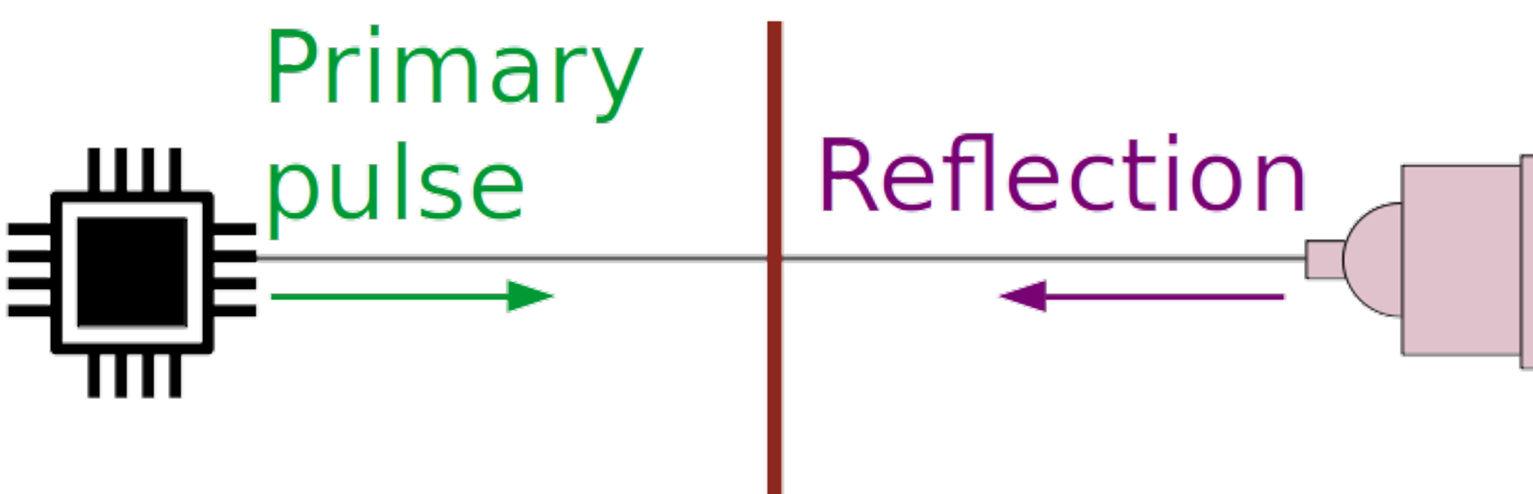
\includegraphics[width=1.1\textwidth]{commissioning/fig_commissioning/scheme_reflecto.pdf}
    \captionsetup{justification=centering}
    \caption{Normal reflection at PMT divider.
      \label{subfig:reflecto_normal}}

  \end{subfigure}
  \hfill
  \begin{subfigure}[b]{0.3\textwidth}
    \centering
    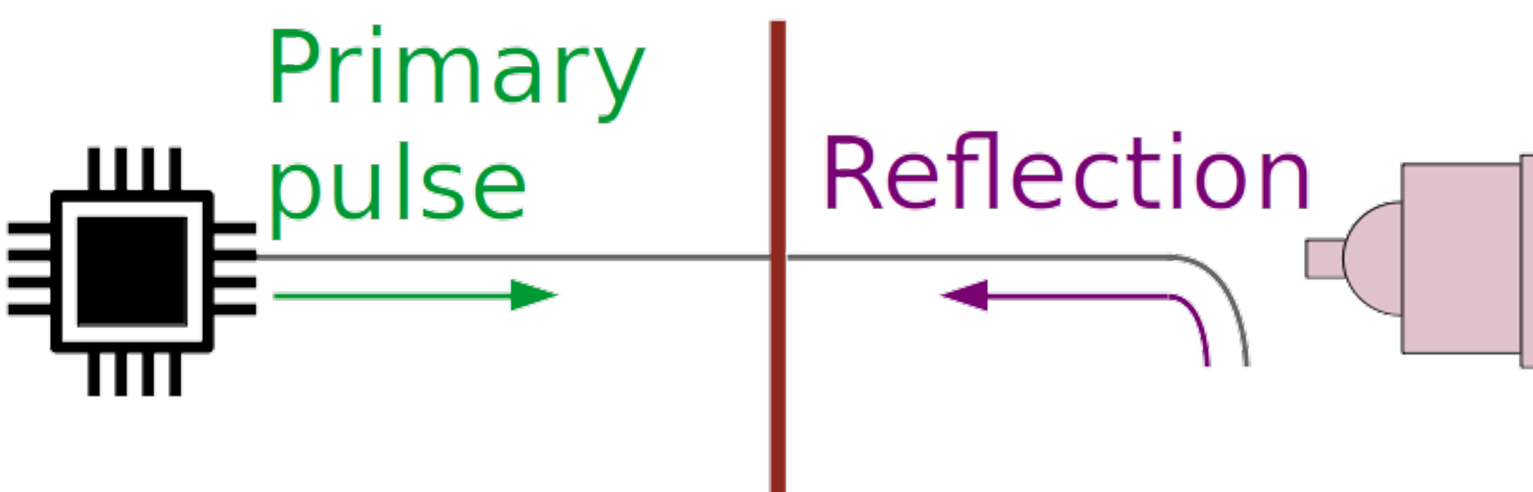
\includegraphics[width=1.1\textwidth]{commissioning/fig_commissioning/scheme_reflecto_1.pdf}
    \captionsetup{justification=centering}
    \caption{Cable not connected at PMT.
      \label{subfig:reflecto_pmt}}

  \end{subfigure}
  \hfill
  \begin{subfigure}[b]{0.3\textwidth}
    \centering
    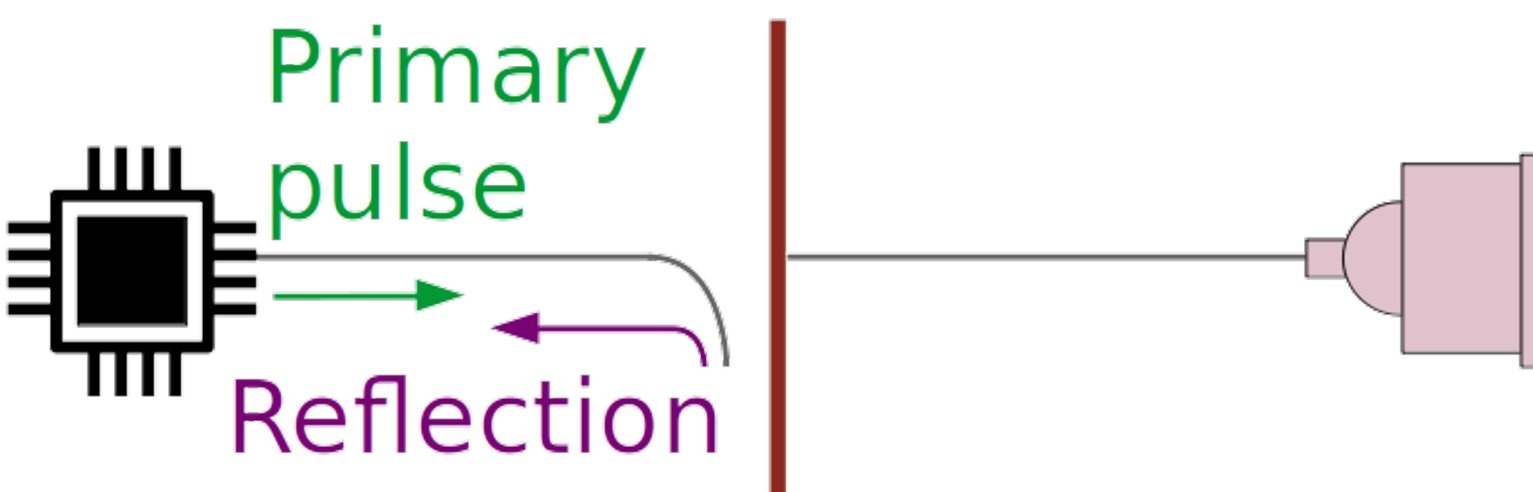
\includegraphics[width=1.1\textwidth]{commissioning/fig_commissioning/scheme_reflecto_2.pdf}
    \captionsetup{justification=centering}
    \caption{Cable not connected at patch panel.
      \label{subfig:reflecto_pp}}

  \end{subfigure}
  \caption{A representation of pulses sent in a cable for the reflectometry analysis is given.
    The electronic boards are symbolised by the black chip, and the patch panel by the red vertical bar.
    Three scenario where a primary pulse is sent in one cable (represented in grey), are represented.
    (a) The cable is well connected at the patch panel and at the PMT. The signal reflects at the PMT divider.
    (b) The cable is not connected at PMT and the signal is reflected at the end of the cable.
    (c) The cable is not connected at patch panel and the signal is reflected at the end of the external cable.\label{fig:reflecto_scheme}}

\end{figure}
Then the signal travels back from the PMT to the electronic board channel, where it is recorded by the acquisition.
We called this recorded reflected pulse \emph{secondary} pulse.
An example of the total recorded signal is displayed in Fig.~\ref{subfig:total_waveform}.
In order to accumulate enough statistics, we send thousands of pulses in each coaxial cable.
The analyses of the shape and of the arrival time of those secondary pulses for each channel is called \emph{reflectometry}, and allow us to check the coaxial cable conditions and to control their lengths.

\subsection{Pulse timing: controlling cable lengths}
\label{subsec:timing}

The first step of this analysis is to experimentally determine the length $l_{j}^{m}$ for all signal cables $j$ installed on the demonstrator.
This length is defined as
\begin{equation}
  l_{j}^{m}= 0.5\,t_{j}\,v_{p}\, ,
\end{equation}
where $t_{j}$ stands as the time made by the electrons to do a round trip between one electronic channel and one PMT, and $v_{p}$ is the velocity of electrons in the coaxial cables, which can be expressed as a fraction of light speed in vacuum, $c$.
The time difference $t_{j}$ between the primary pulse and the secondary pulse is written as
\begin{equation}
  t_{j} = \braket{t_{\text{secondary pulse}}-t_{\text{primary pulse}}}_{p} \, \text{,}
\end{equation}
$\braket{}_{p}$ being the average over all pulses sent in one single cable $j$.
The velocity $v_{p}$ is supplied by the cable manufacturer as
\begin{equation*}
  v_{p}=\frac{c}{\sqrt{\epsilon_{r}}}\,\text{,}
\end{equation*}
with $\epsilon_{r}$ the relative dielectric constant of the material.
Therefore, this celerity depends on the components.
For the coaxial cables chosen in the demonstrator design, the data sheet of the cable gives ${v_{p}=0.69\,c}$.
A study is performed to verify experimentally the value of $v_{p}$.
Three cables of different lengths are measured with a precision of $1$ cm.
A thousand of primary pulses are sent in each of the three cables, then the time for each secondary pulse is recorded.
At the end, we have three independent measures of the velocity $v_{p}$ in the used coaxial cables.
On Fig.~\ref{fig:celerity} is displayed the lengths $l_{j}$ as a function of the times $t_{j}$.
\begin{figure}[h]
  \centering
  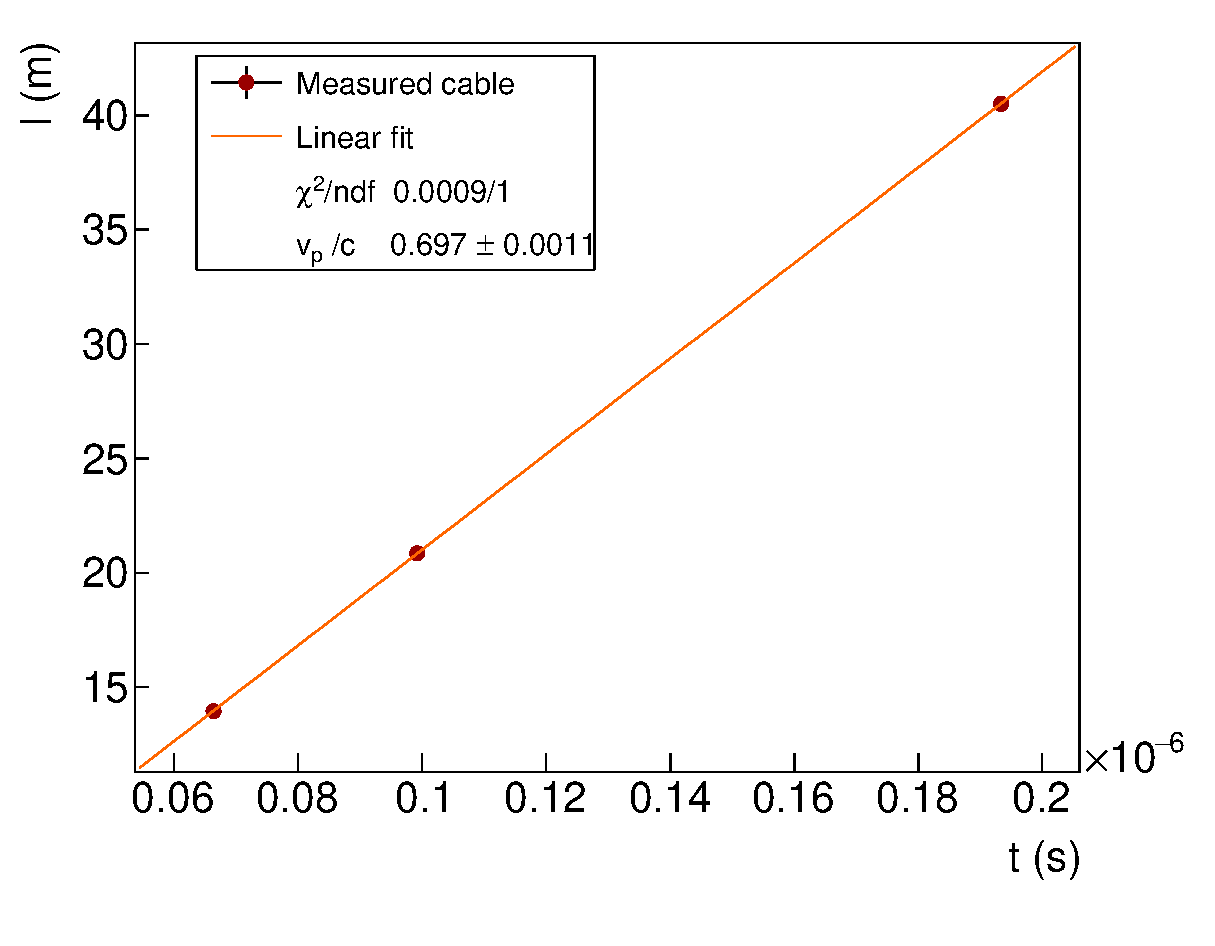
\includegraphics[width=15cm]{commissioning/fig_commissioning/celerity.eps}
  \caption{Three different lengths $l_{j}$ of cables are measured.
    Pulses are sent inside all cables.
    The lengths $l_{j}$ are plotted as a function of the time differences $t_{j}$ between primary and secondary pulses.
    The value of $v_{p}/c$ fitted from the data points is displayed.
    This value of $0.697\pm 0.0011$ shows the compatibility with the one supplied by the constructor, of $0.69$ c.
    \label{fig:celerity}}
\end{figure}
The fitted value of $v_{p}/c = 0.697\pm 0.0011$ is displayed and shows a compatibility up to $7\sigma$ with the data sheet.

As we want to determine the time interval $t_{j}$, we have to define what is the \emph{time} of a pulse.
In this analysis, we use a technique called Constant Fraction Discriminator (CFD), providing an amplitude-independent information about time of a pulse.
This algorithm aims at tracking a signal and defining its time arrival at a given fraction $f$ of its maximal amplitude.
The two main advantages of this technique is that it provides an efficient rejection of the noise in the acquisition window, and gives a good resolution on the measured time.
Nevertheless, the possible influence of the chosen value for the $f$ parameter on this time resolution has to be investigated.
We perform such a study in Sec.~\ref{subsec:CFD}.
We concluded that the highest precision on the time measurement arises for $f = 40\%$, and we adopt this value for the following analysis.
A graphic representation of the CFD time search is given in fig.~\ref{subfig:zoom_secondary}.
\begin{figure}[h]
\centering
\begin{subfigure}[t]{0.7\textwidth}
  \centering
  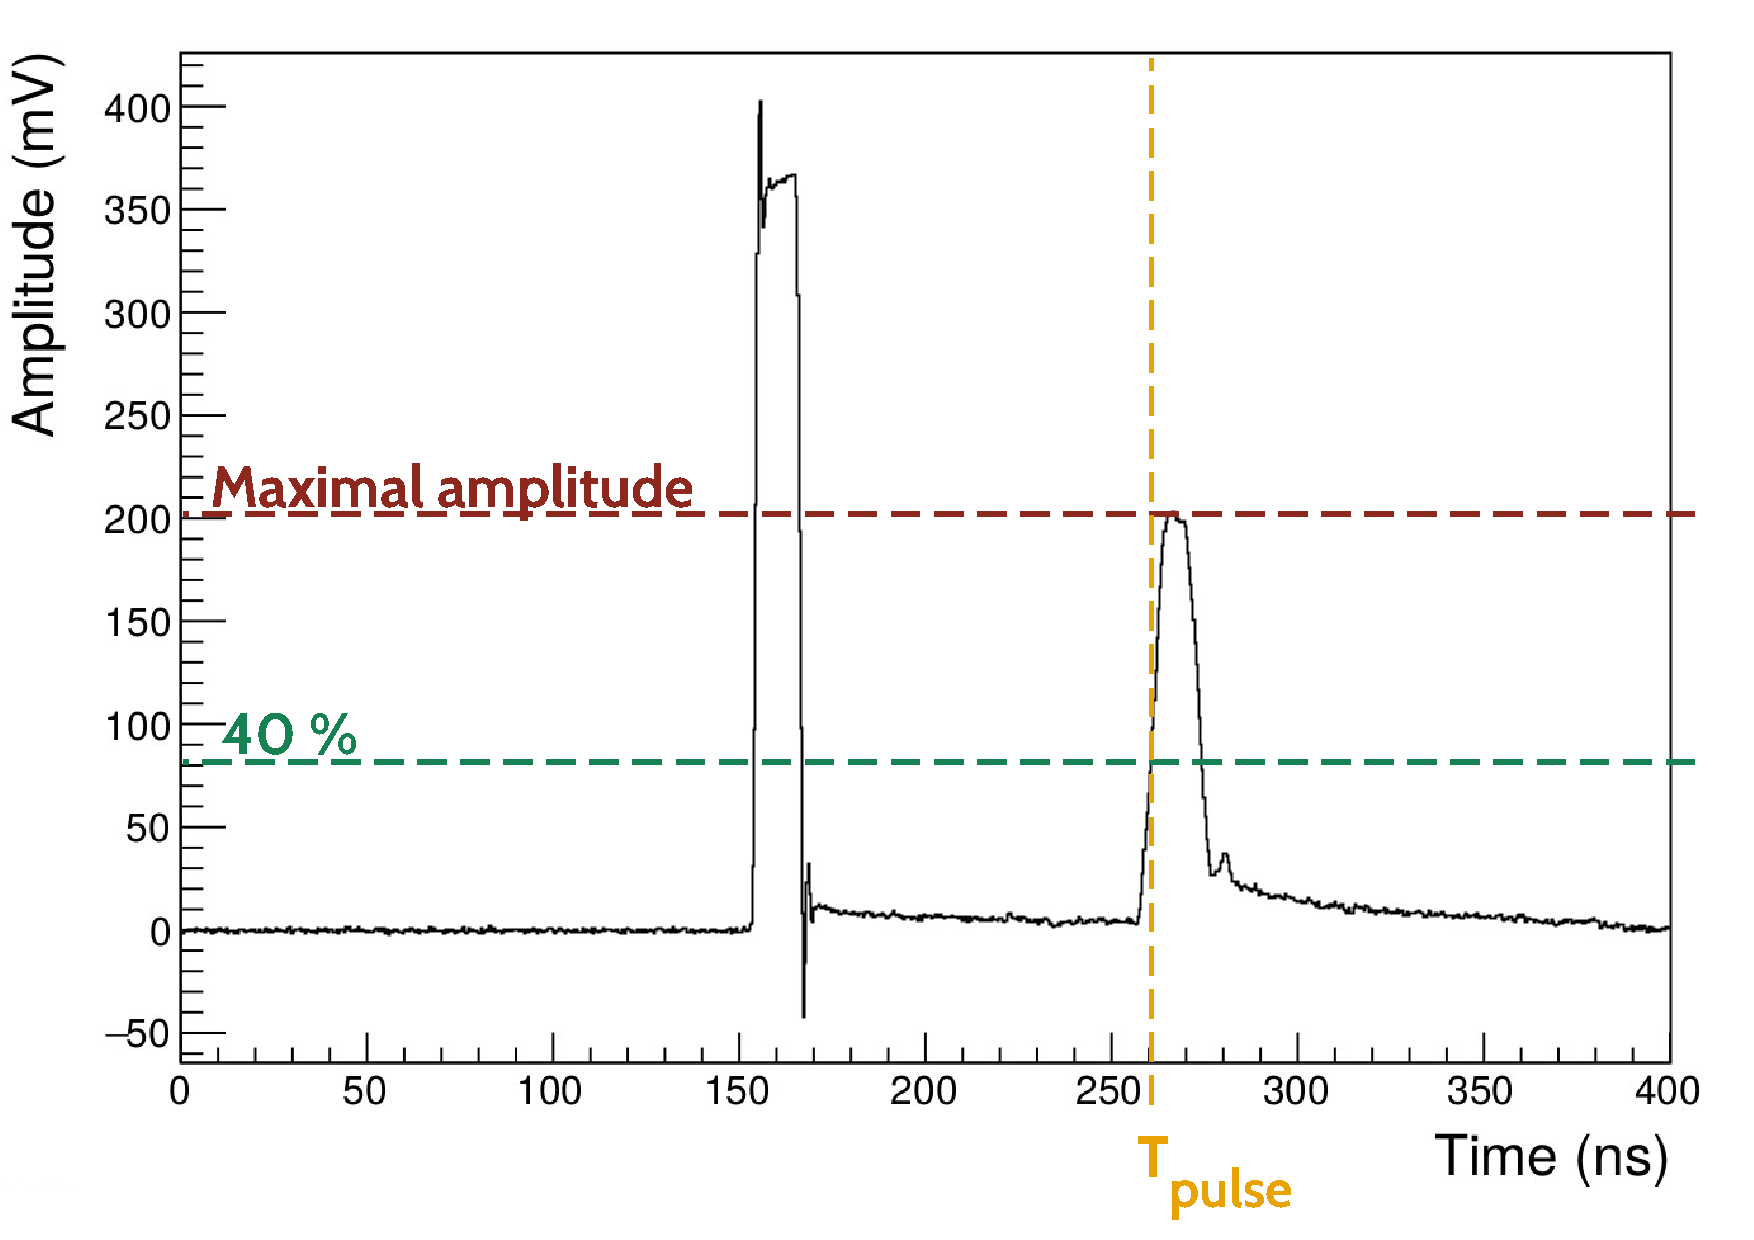
\includegraphics[trim={1.2cm 3.5cm 1.7cm 3.1cm},clip,width=1\textwidth]{commissioning/fig_commissioning/CFD_example.pdf}
  \captionsetup{justification=centering}
  \caption{Total recorded waveform
    \label{subfig:total_waveform}}
\end{subfigure}
\hfill
\begin{subfigure}[t]{0.7\textwidth}
  \centering
  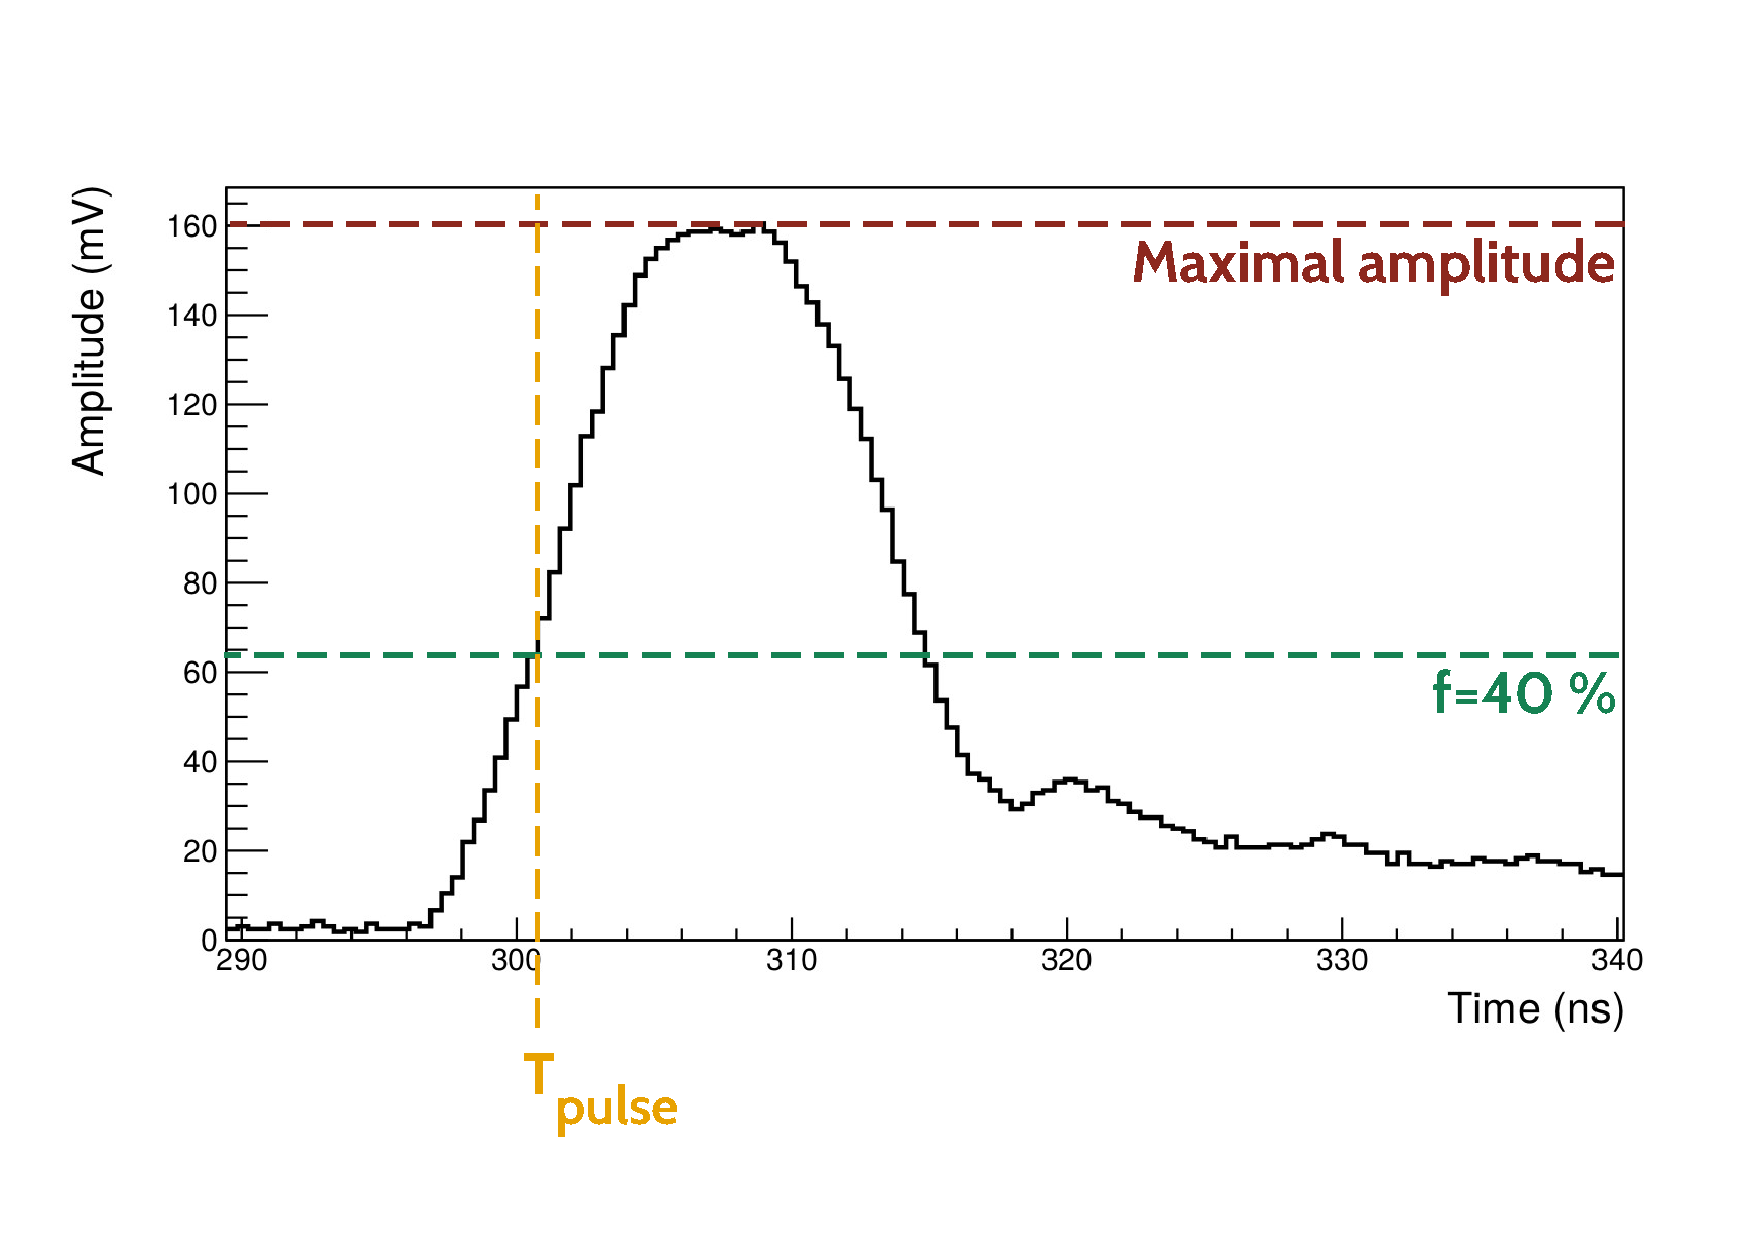
\includegraphics[trim={1.2cm 1.5cm 1.7cm 3.1cm},clip,width=1\textwidth]{commissioning/fig_commissioning/CFD_example_zoom.pdf}
  \captionsetup{justification=centering}
  \caption{Zoom on secondary pulse
    \label{subfig:zoom_secondary}}
\end{subfigure}
\caption{(a) Total recorded waveform: primary pulse (left) and secondary the pulse (right).
  (b) Zoom on the secondary pulse.
    A representation of time computed with a Constant Fraction Discriminator (CFD) is provided.
    Its maximal amplitude (red dotted line) and its fraction for $\text{f}=40\%$ (green dotted line) are displayed.
    The time $\text{T}_{\text{pulse}}$ (orange dotted line) represents the time of arrival of the secondary pulse computed with CFD, with the fraction $\text{f}=40\%$.
  \label{fig:CFD}}
\end{figure}
As we want to measure the installed cable lengths $l^{m}_{j}$, and compare them to the initially designed ones, $l^{d}_{j}$, we define the length difference $\Delta L_{j}$ as:
\begin{equation}
  \Delta L_{j} = l^{m}_{j}-l^{d}_{j}\, .
\end{equation}
On Fig.~\ref{fig:LengthDiff} is displayed the distribution $\Delta L$ for all the measured lengths.
\begin{figure}[h]
  \centering
  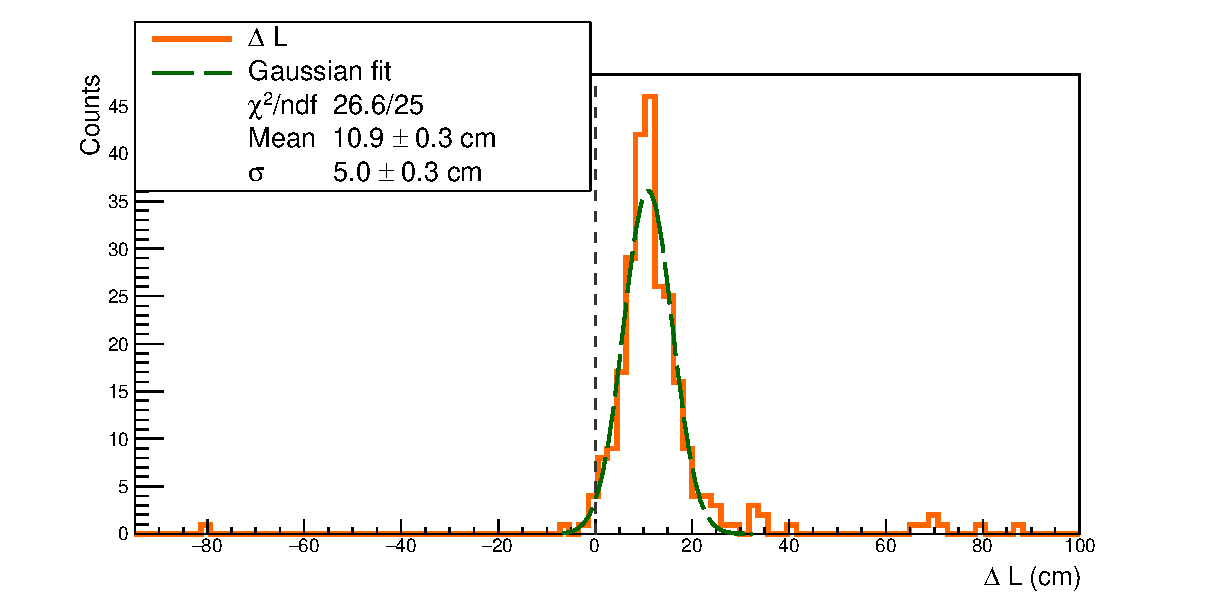
\includegraphics[width=15cm]{commissioning/fig_commissioning/length_diff.eps}

  \caption{The distribution of difference between the measured lengths $l^{m}$ and the expected lengths $l^{d}$ is displayed in orange solid line.
    The black dashed line represents the case where $l^{m}_{j} = l^{d}_{j} \;\forall j$.
    The Gaussian fit (green dashed line) presents a mean of $10.9 \pm 0.3$ cm.
    Some data points considered as outliers are beyond $3\sigma$.
    \label{fig:LengthDiff}}
\end{figure}
In hypothetical perfect conditions, all the cables should fit the design length, in other words, $l^{d}_{j} = l^{m}_{j}$.
Consequently the $\Delta L$ distribution should a peak at zero, as materialised by the black dashed line.
However, in real conditions, the measured length can be different from the designed one, leading the $\Delta L$ distribution plotted in orange solid line.
We conclude that the observed cable length $l^{m}$ differs from $l^{d}$ by $+10.9\pm 0.3$ cm, meaning that cables are longer than expected in average.
This may reveal a bias coming from the device used to cut the cables.
In fact, during cable cutting work, we noticed that the cutting device had a tendency to slip, probably leading to cables with extra lengths.
We assumed the cutting device has a given probability to slip for one meter of cable.
If this is the case, the probability for the device to give extra length should increase with the cable length.

To verify this assumption, we plot on Fig.~\ref{fig:CutBias} the length difference $\Delta L$ as a function of the initial design length $l^{d}$ (cyan).
From those data points, we compute a linear fit (orange solid line), parameterised as $y = \alpha x + \beta$, revealing that the cutting device presents two different biases.
\begin{figure}[h]
  \centering
  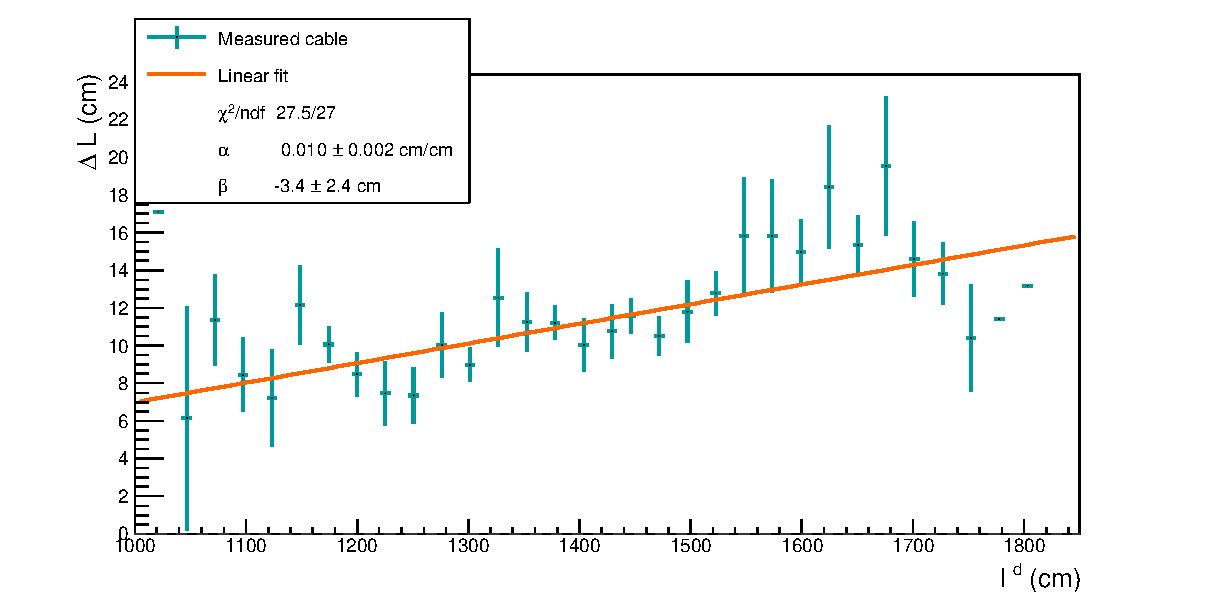
\includegraphics[width=15cm]{commissioning/fig_commissioning/cut_biais.eps}

  \caption{$\Delta L$ is plotted with $l^{d}$ (cyan), where $l^{d}$ is averaged for all the lengths designed to have the same value, being at the origin of vertical error bars.
    In black dashed line is represented the case where $l^{m} = l^{m}$.
    Data points are fitted by $\alpha x + \beta$, with $\alpha > 0$ and $\beta < 0$, revealing the two biases of the cutting device.
    \label{fig:CutBias}}
\end{figure}
The value of $\beta$ shows that the cutting device systematically took away $3.4$ cm of each cable.
Nevertheless, as the shortest cable was designed to be 10 meters long, there are no important consequences of this bias on the length difference $\Delta L$.
Besides, the slope $\alpha = 0.010\pm 0.002$ of the linear fit reveals that the cutting device adds one centimetre for every meter of cable, being compatible with the hypothesis on the cutting device sliding.
Hopefully this bias is not problematic as it makes most of the actual cable lengths longer than the design, while shorter lengths could have lead to systematic connection issues to PMTs.
However, we notice that a few cables have been cut too short by mistake, the worse of them being $80$ centimetres shorter than expected.
Fortunately, this cable  was successfully connected to PMT despite this deficit.
On the contrary, few cables have a large extra length.
This probably is due to human punctual mistakes on top of the observed bias, but without any strong consequences for the calorimeter operation.
In conclusion, no important mistakes have been made when cutting cables, and we had no issue for connecting the only problematic cable.

If the main goal of this study is to check the lengths of coaxial cables, it also aims at correcting the time of recorded events, from the time made by the signal to travel from a PMT to an electronic channel.
taking into account the time for the signal to travel through cables.
This become possible with the reflectometry study we performed.
Knowing real lengths of cables and using the celerity of the signal, we deduce the time needed for the signal to travel from one given PMT divider to the electronic boards.
Then we can correct event times.

As explained previously, the time $t_{j}$ gives information about the length of the cable $j$.
We remind the coaxial cables are divided in two parts, one external and one internal, both linked by the so-called patch panel.
Thus we can use that travel time to detect possible disconnection of a cable at patch panel.
In fact, if one cable is not connected at the patch panel -- this case is illustrated in Fig.~\ref{subfig:reflecto_pp}, -- the pulse reflects at the end of the external cable part, going back to the electronic board.
This very short time, giving information about the location of the reflection, is used to tag a patch-panel disconnection.
Then, a simple check onsite can confirm this observation, and the external part of the cable can be connected to the patch panel.
\newline

This study allowed us to control and record the lengths of all coaxial cables installed on the SuperNEMO demonstrator at LSM, and gave information on the status of cable connections at patch panel.
We also have understood the main results on measured cable lengths and the functioning and biases of the cutting device that we used.

\subsection{Signal attenuation}
\label{subsec:attenuation}
The attenuation of an electric signal is a problem common to all electronic fields, and comes from the charge loss of an electromagnetic wave travelling in a medium.
%% Then, another test for controlling the cable condition is to check if this attenuation matches
%% the expectations (i.e. the attenuation per metre of cable given by constructor).
%% The signal attenuation car be define in two different ways:
%% \begin{itemize*}
%% \item using the signal amplitude ratio
%% \end{itemize*}
For a coaxial cable, this attenuation mainly depends on the signal frequency $f$ in MHz and on the cable characteristics.
For the coaxial cables, the theoretical linear attenuation $\alpha_{\text{att}}^{\text{th}}$, so be it the attenuation by metre of cable in dB/m, is supplied by the constructor as
\begin{equation}
  \alpha_{\text{att}}^{\text{th}} = f\sqrt{\epsilon}(\frac{a}{\sqrt{f}}+b)\,,
\end{equation}
where the factor $a$ depends on the diameter of the dielectric material on one side, and of the diameter of the conductor material on the other side, and where $b$ is function of the dielectric loss factor, characterising the material's dissipation of electromagnetic energy.
For the used coaxial cables, and with a frequency $f$ of few GHz for the signal pulses sent in cables, we calculate this attenuation as $\alpha_{\text{att}}^{\text{th}} = 1.22$ dB/m.
In a more general manner, the attenuation of a signal in dB is defined with the decimal logarithm of a power ratio.
We use this definition to determine the attenuation in the framework of the reflectometry analysis, defining the attenuation $\mathcal{A}$, for a given length of cable $l$, as
\begin{equation}
  \mathcal{A}=10\log_{10}\frac{V_{\text{primary pulse}}}{V_{\text{secondary pulse}}} \,\text{,}
\end{equation}
where $V_{i}$ is a quantity representing the intensity of the signal.
$V$ can correspond to the maximal amplitude of the pulse, as well as the \emph{integrated charge} of the pulse, defined as the amount of current received by the acquisition over a given time window.
As the provided data sheet does not specify the attenuation of which quantity (amplitude or charge) represents $\alpha_{\text{att}}^{\text{th}}$, we decide to investigate both in the following.
Then, we define the linear attenuation $\alpha_{\text{att}}^{\text{R}}$, measured by reflectometry in dB/m, with
\begin{equation}
  \mathcal{A} = f_{r}+\alpha_{\text{att}}^{\text{R}}\,l\,,
\end{equation}
with $f_{r} = -10\log_{10}R$, where $R$ is the reflection factor characterising the pulse reflection on the PMT divider.
In fact, as the circuit is opened, the pulse is reflected at the PMT divider, but only partially.
A part of the signal is not reflected but lost through the divider.
This reflection is characterised by $R$, which is function of the impedance $Z_{c}$ of the cable, and of the impedance $Z_{d}$ at the divider level, where the pulse is reflected.
It is written as
\begin{equation}
  R = \frac{Z_{d}-Z_{c}}{Z_{d}+Z_{c}}\,,
\end{equation}
where we have the limit
\begin{equation}
  \lim_{Z_{d} \to \infty} f_{r} = 0 \text{ and } R=1\,,
\end{equation}
expressing a total reflection occurring when the impedance at the PMT divider is infinite.
The main goal here is to determine the value of $\alpha_{\text{att}}^{\text{R}}$, using the reflectometry data, and to compare it with $\alpha_{\text{att}}^{\text{th}}$.
Moreover, the impedance $Z_{d}$ value at PMT divider can be estimated from the determination of $f_{r}$.
On Fig.~\ref{fig:attenuation} is shown the linear dependence between the attenuation $\mathcal{A}$ and the cable length $l$, and two data set are presented.
The cyan scattered markers represent the attenuation calculated from the amplitude ratio $A_{\text{primary pulse}}/A_{\text{secondary pulse}}$, and the magenta markers correspond to the attenuation calculated from the charge ratio $Q_{\text{primary pulse}}/Q_{\text{secondary pulse}}$.
The amplitude $A_{i}$ is given in mV and the charge $Q_{i}$ in mV.ns.
\begin{figure}[h]
  \centering
  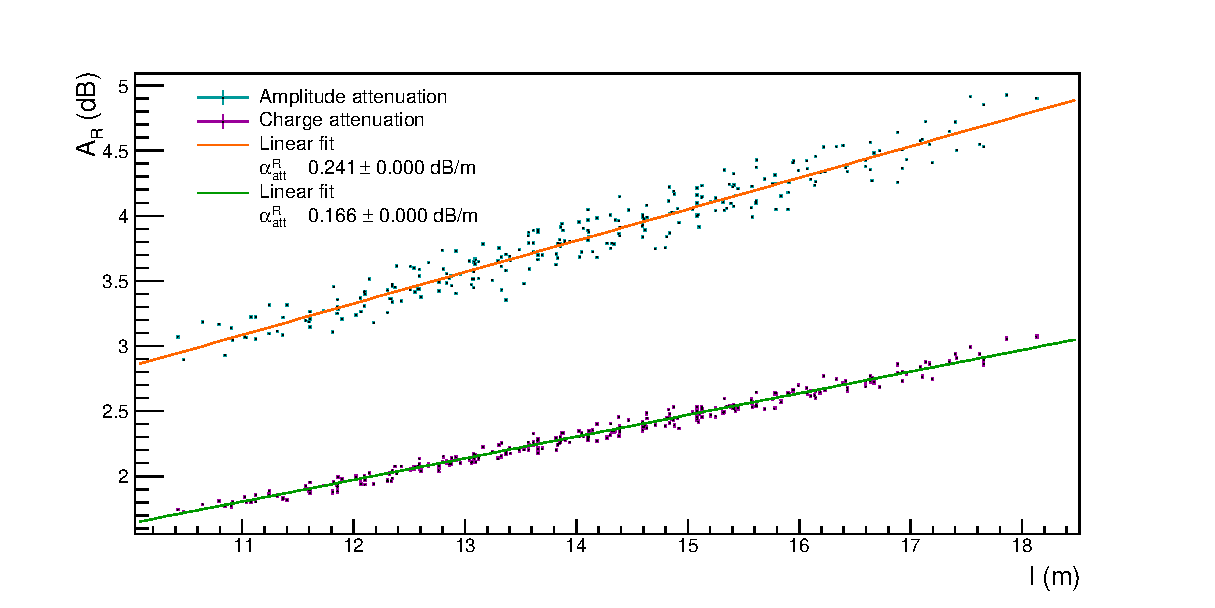
\includegraphics[width=15cm]{commissioning/fig_commissioning/attenuation_length.eps}
  \caption{The amplitude $\mathcal{A}$ is displayed as a function of the measured cable length $l$.
    The data set calculated with the amplitude (charge) is given in cyan (magenta) and fitted by a linear function in orange (green).
    The values of the slope, which represent the linear attenuation of the coaxial cables in dB/m, are respectively $\alpha_{\text{att}}^{\text{R, amp}} = 0.241\pm 0.000$dB/m and $\alpha_{\text{att}}^{\text{R, ch}} = 0.166\pm0.000$dB/m.
    The two $y$-intercept values, which represent the reflection of the pulse on the PMT divider, are $f_{r}^{amp} = 0.402\pm 0.032$ dB and $f_{r}^{ch} = -0.020\pm 0.013$ dB.
    \label{fig:attenuation}}
\end{figure}
The values of $\alpha_{\text{att}}^{\text{R}}$ and $f_{r}$, for both amplitude and charge cases, are displayed in the legend.
Firstly, the two linear fits reveal that, whether calculated with the amplitude, or with the charge, the linear attenuation $\alpha_{\text{att}}^{\text{R}}$ is smaller than the calculated one $\alpha_{\text{att}}^{\text{th}}$ (for the amplitude case, $\alpha_{\text{att}}^{\text{th}}\simeq 5\times \alpha_{\text{att}}^{\text{R, amp}}$, and for the charge case $\alpha_{\text{att}}^{\text{th}}\simeq 7\times \alpha_{\text{att}}^{\text{R, ch}}$).
That means the signal is less affected, when transmitted by the cable, than expected.
Secondly, the attenuation in charge is less important that the attenuation in amplitude.
This can be easily explained: as it is integrated over time, the charge is a quantity less affected by amplitude variations that the amplitude itself.
For the same reason, the charge data set points are less spread than the amplitude ones, meaning that we are less sensitive to cable length variations when using the charge quantity.


This work achieved, we want to verify if no cable was damaged after installation.
Reflectometry also aimed at checking cable conditions by performing waveform shape analysis on secondary pulses.

\subsection{Pulse shape analysis}
\label{subsec:pulse_shape}
On Fig.~\ref{fig:CFD} is displayed an example of \emph{normal} pulse, which corresponds to the case represented in Fig.~\ref{subfig:reflecto_normal}.
In this case, the pulse sent in the cable travels to the PMT, and goes back to the acquisition after reflection on the divider.


\subsection{Comparison with $^{60}$Co}



\section{Calibrating the electronic boards}
\label{sec:TimeSynchroFEB}

\subsection{Principle}
\subsection{Measuring the time offset of front end boards}
\subsection{Results}







\chapter{Characterisation of the calorimeter time resolution}

The precise knowledge of the different particle interaction times in the optical modules of the SuperNEMO calorimeter is important to better understand and reject background.
For example, the study of electron time-of-flight allows us to distinguish internal events (coming from source foils) from external events (PMTs, scintillators, tracker...).
\newline

In this chapter we present different studies conducted in order to characterise the time response of the SuperNEMO optical modules.


%%%%%%%%%%%%%%%%%%%%%%%%%%%%%%%%%%%%%%%%%%%%%%%%%%%%%%%%%%%%%%%%%%%%%%%%%%%%%%%%%%%%%%%%%%%%%%%%%%%%%%%%%%%%%%%%%%%%%%%%%%%%%%%%
\section{Time calibration with a Cobalt source}
\label{sec:CoSource}
Cobalt $60$ decays through $\beta^{-}$ decay, emitting an electron with a maximum energy of $318$ keV, into an excited state of the stable nickel-60.
A simplified decay scheme for this atomic element is given in Fig.~\ref{fig:Co_decay_scheme}.
\begin{figure}[h]
  \centering
  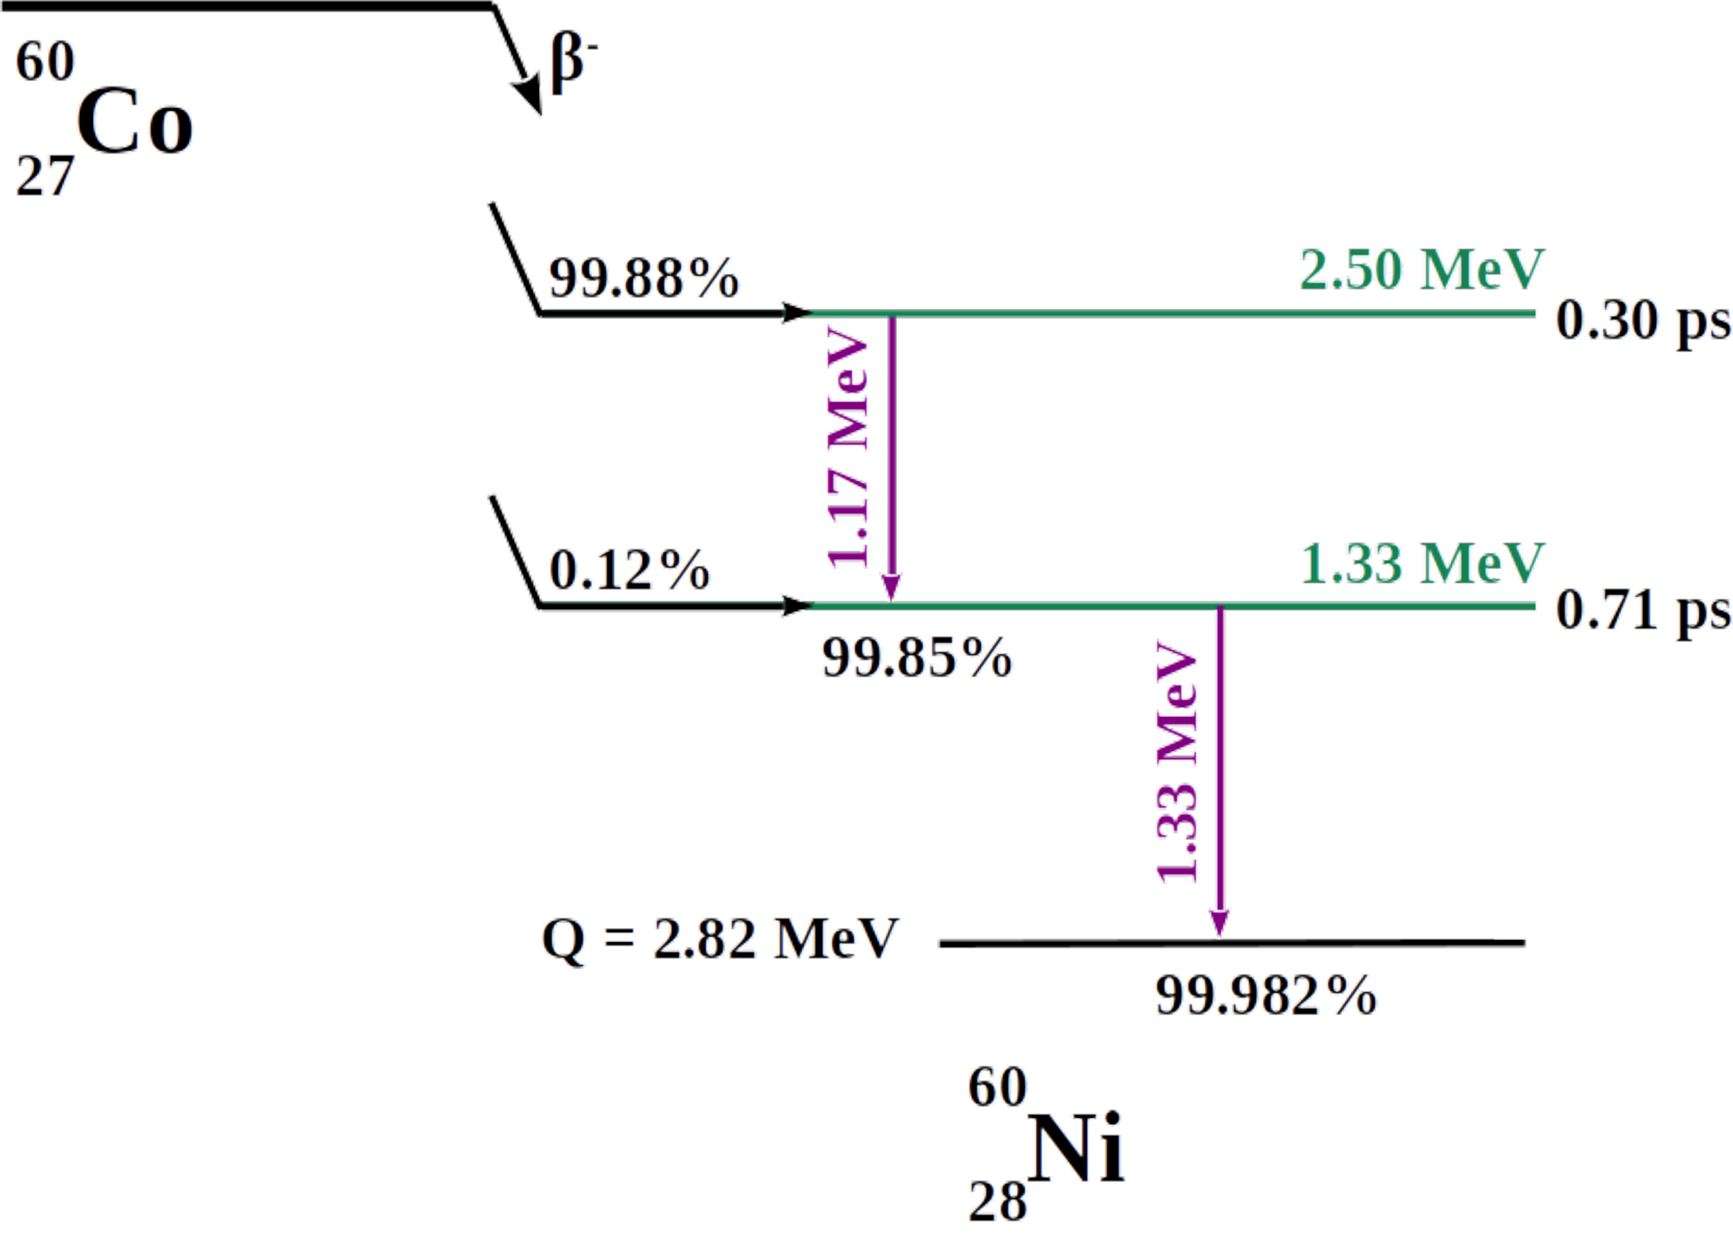
\includegraphics[width=10cm]{commissioning/fig_commissioning/Co_decay_scheme.pdf}
  \caption{A simplified decay scheme for Cobalt $60$.
    The Cobalt decays, through $\beta^{-}$, predominantly to the $2.50$ MeV state.
    Then, two $\gamma$'s (whose energy levels are represented in green) are emitted in $99.66$\% of the cases.
    The two photons have an energy of $1.17$ MeV and $1.33$ MeV, respectively.
    As the life times of these two energy levels are short ($<1$ ps), the two photons can be considered as emitted in coincidence.
    We use this property to calibrate in time the demonstrator optical modules.
    \label{fig:Co_decay_scheme}}
\end{figure}
From this energy level, a transition into another excited state takes place with emission of a $1.17$ keV photon, then the ground state is reached whith emission of a photon of $1.33$ keV.
The life times of these two energy levels are very short, so the two photons are considered as emitted in coincidence with respect to the expected timing precision of the calorimeter.
The goal of this analysis is to calibrate in time the SuperNEMO optical modules with a Cobalt $60$ source, exploiting the time characteristic of those two emitted photons.

\subsection{Time response of optical modules}
\label{sec:OMtimeResponse}

A calorimeter block of SuperNEMO, composed of a scintillator and a photomultiplier, measures the scintillation light generated by the interaction of incoming particles.
The energy of the incident particle stopping in the scintillator (photon, electron, alpha...) is fully absorbed.
The photons produced by the scintillating material are converted in electrons at the photomultiplier photocathode.
After amplification, electrons are collected by the anode which delivers an electric signal whose charge is proportional to the initial amount of incident photoelectrons.
This signal is then transmitted, via the PM voltage divider, to the electronic readout, where the signal is sampled.
Energy and time of arrival of the incident particle can be extracted from the signal waveform analysis.
Especially, the arrival time of the particle, defined in Fig~\ref{subfig:zoom_secondary} in Sec.~\ref{sec:reflecto}, can be estimated.
Each step, from the incident particle interaction inside the scintillator, to the signal sampling at the electronic readout, can have an impact on this arrival time measurement.
On this section, we focus on the time resolution $\sigma_{t}$ induced by the optical module, and written as
\begin{equation}
  \sigma_{t}=\sqrt{\sigma_{t,\text{sc}}^{2}+\sigma_{t,\text{PM}}^{2}}\,,
  \label{eq:Co_sigma_t}
\end{equation}
where the two terms $\sigma_{t,\text{sc}}$ and $\sigma_{t,\text{PM}}$ represent the time resolutions of the scintillator and of the PMT, respectively.
We detail the physical origins of those terms.

\subsubsection*{Scintillator time dispersion}
The temporal dispersion $\sigma_{t,\text{sc}}$ in Eq.~\eqref{eq:Co_sigma_t} is based on the  scintillator operating principle.
When a particle interacts in the scintillator, two successive mechanisms of light absorption/re-emission take place.
The excitation of scintillator molecules leads to the creation of fluorescence photons.
Those photons are then absorbed and re-emitted by the POPOP agent at higher wavelengths.
These two processes follow the same temporal distribution
\begin{equation}
\mathcal{N}_{\text{photons}} = A\times e^{-t/\tau}\,,
\label{eq:fluorescence_photons_time}
\end{equation}
with $\mathcal{N}_{\text{photons}}$ the number of generated photons at time $t$, $A$ a normalisation constant and $\tau$ the fluorescence characteristic time of the considered process.

Another important phenomenon comes with the uncertainty on the interaction point location in the scintillator, which depends on the incident particle type.
Depending on whether the incident particle is a photon or an electron, the term $\sigma_{t,\text{sc}}$ has a different contribution on the total time resolution $\sigma_{t}$.
To picture this, we display the radiation length of photons and electrons in polystyrene on Fig~\ref{fig:particle_attenuation}.
\begin{figure}[h]
\centering
\begin{subfigure}[t]{0.48\textwidth}
  \centering
  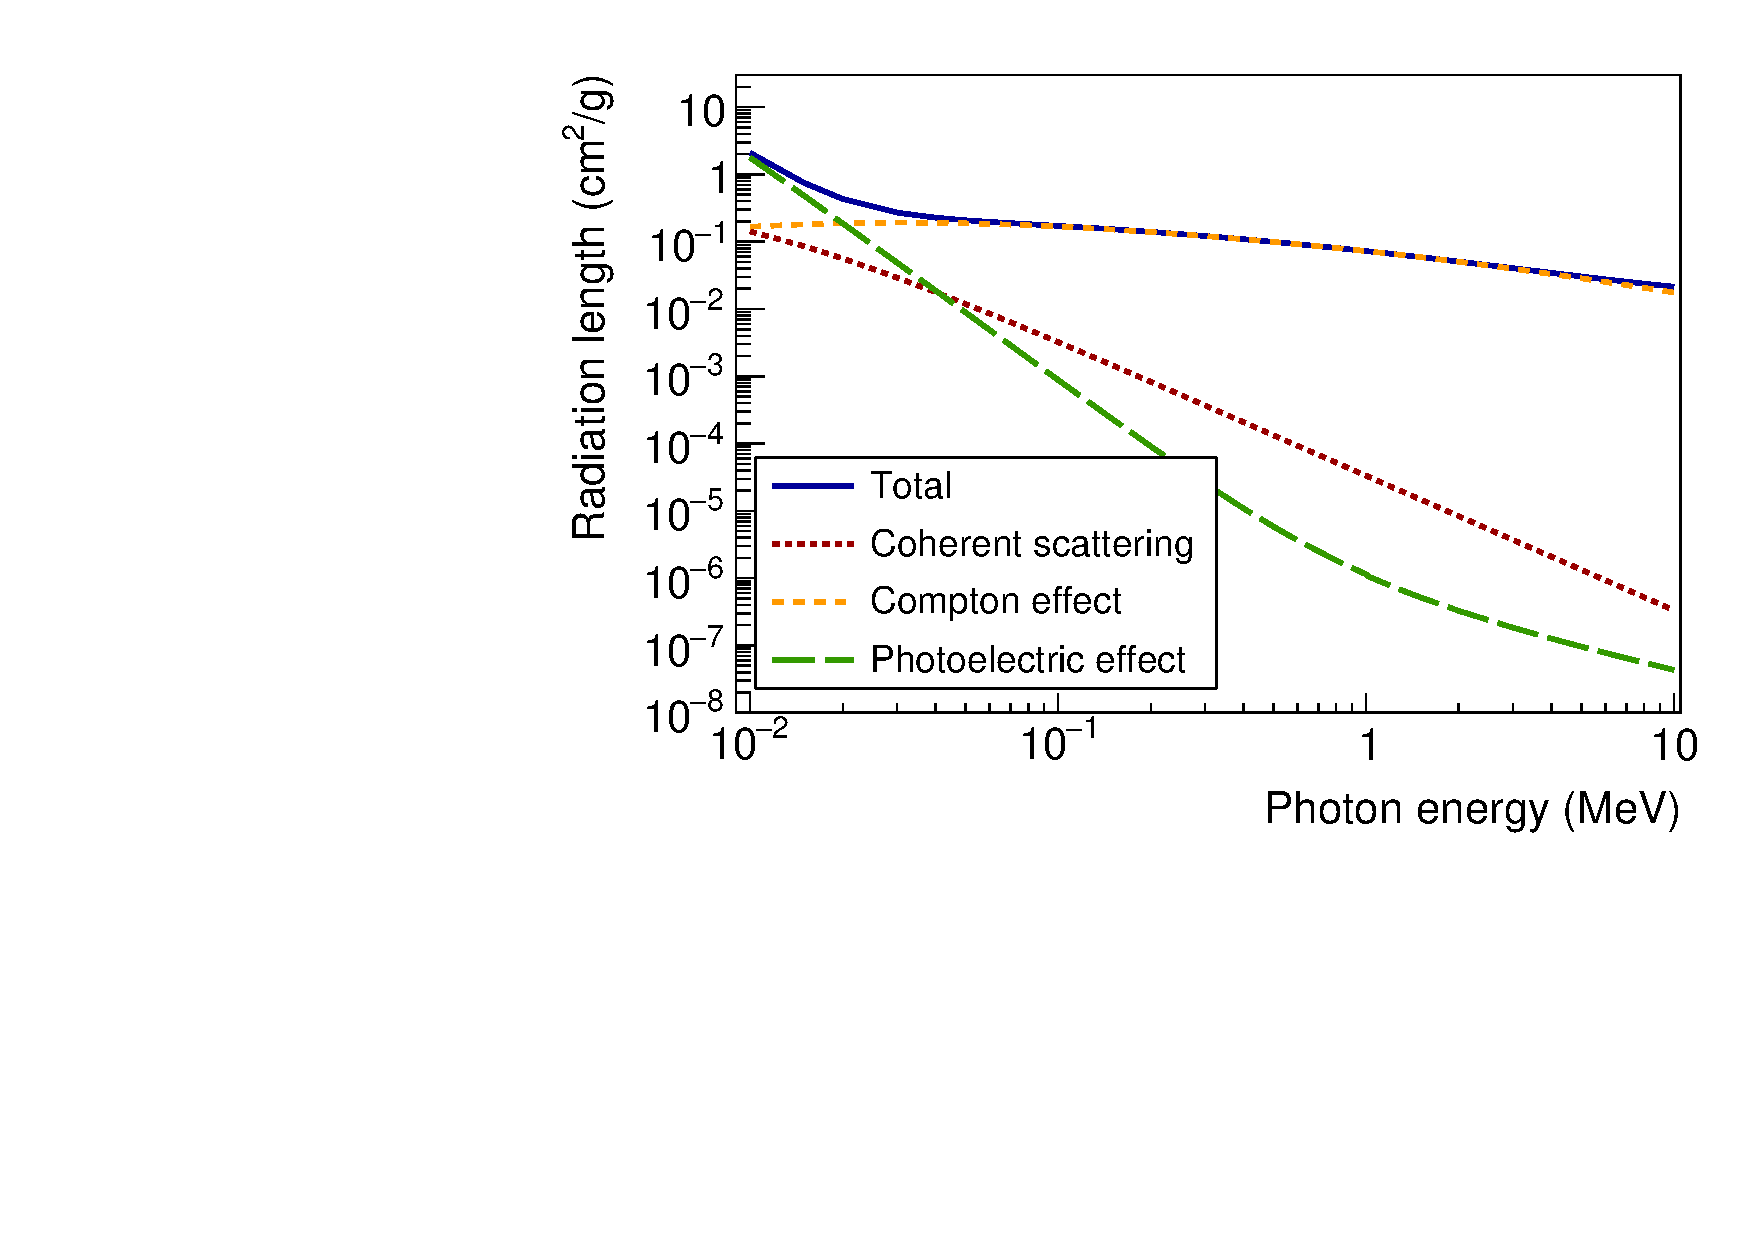
\includegraphics[width=1\textwidth]{commissioning/fig_commissioning/photon_energy_loss.pdf}
  \captionsetup{justification=justified}
  \caption{
    \label{subfig:photon}}
\end{subfigure}
\hfill
\begin{subfigure}[t]{0.48\textwidth}
  \centering
  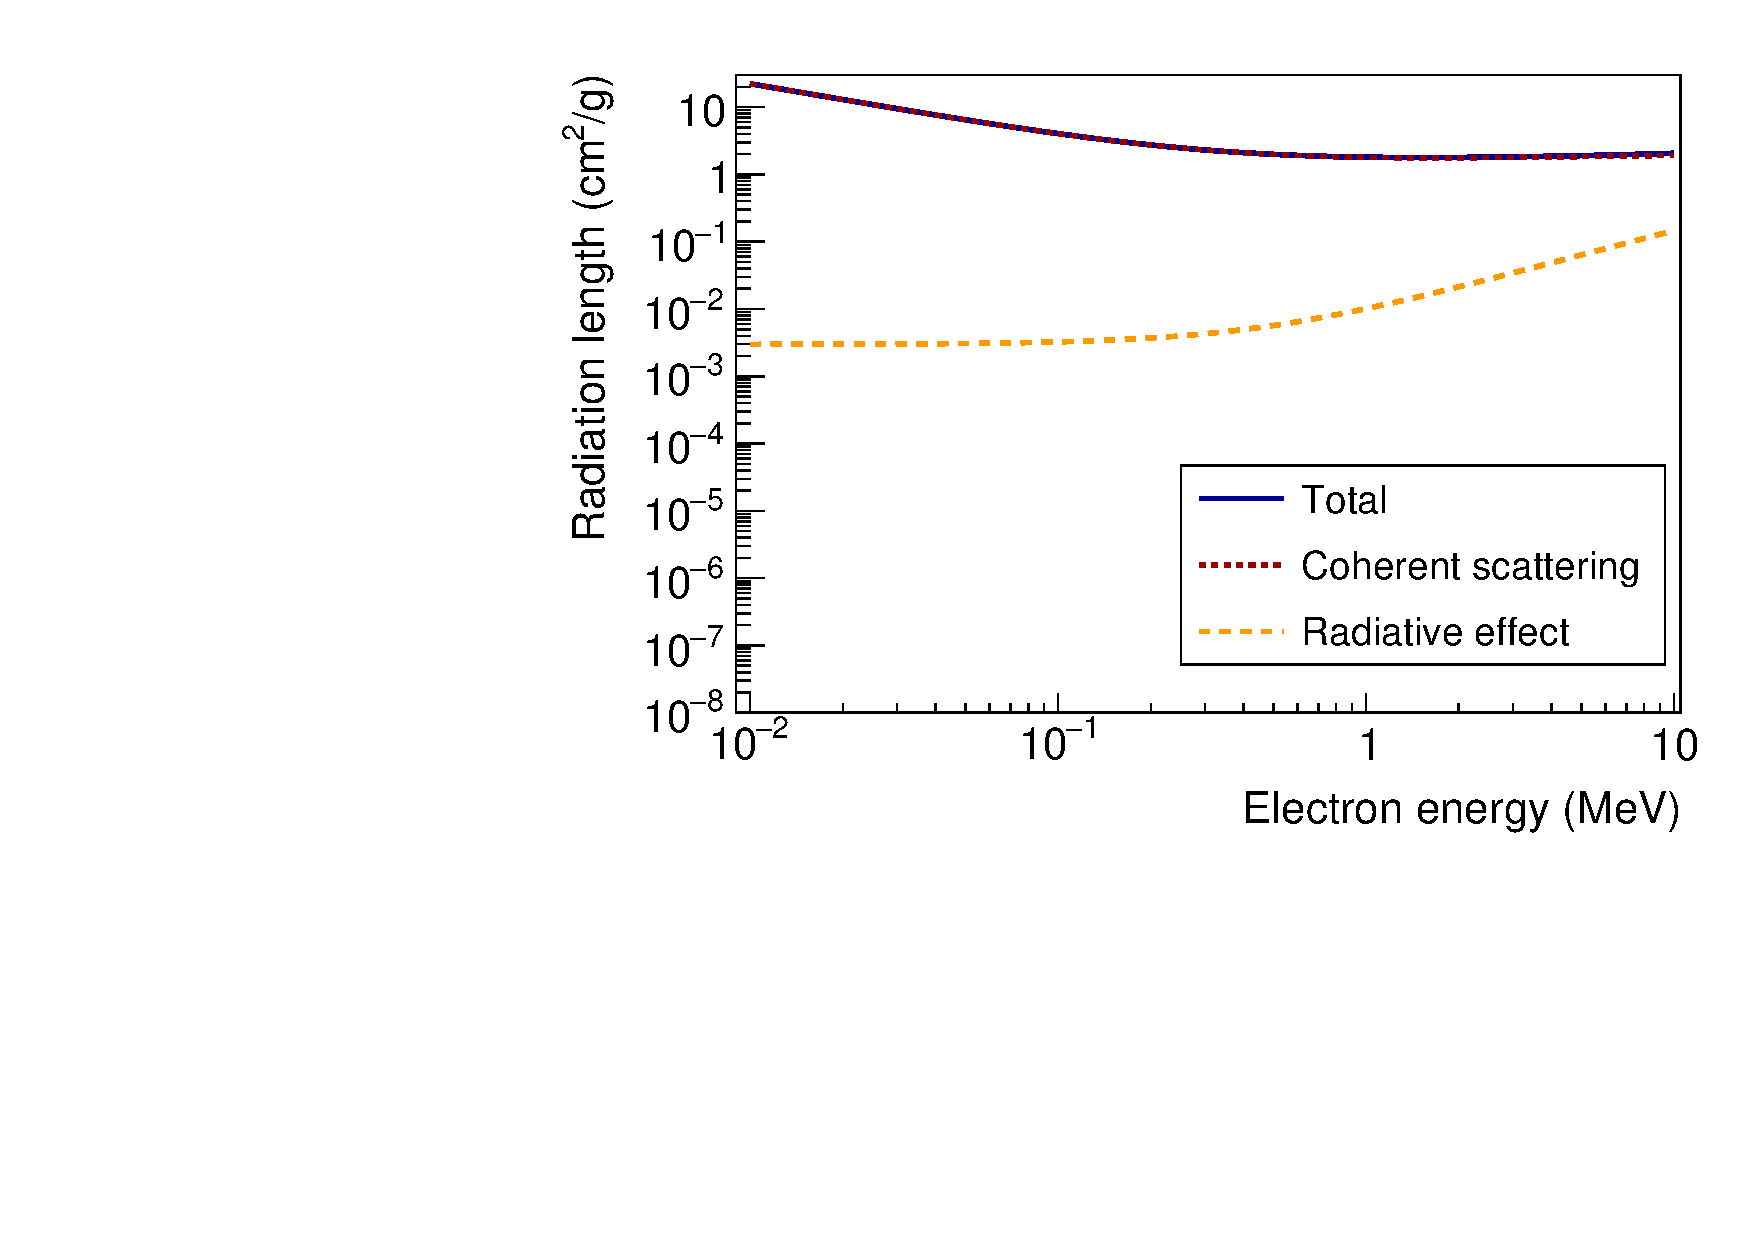
\includegraphics[width=1\textwidth]{commissioning/fig_commissioning/electron_energy_loss.pdf}
  \captionsetup{justification=justified}
  \caption{
    \label{subfig:electron}}
\end{subfigure}
\caption{(a) Cross section of photons in polystyrene: coherent scattering (red dotted line), Compton effect (orange dotted line), photoelectric effect (green solid line) and total contribution (blue solid line).
  (b) Stopping power for electrons in polystyrene: coherent scattering (red dotted line), radiative effect (orange dotted line) and total contribution (blue solid line).
  At the considered energy range $10$ keV $ -\; 10$ MeV, the interaction of photons with matter is dominated by Compton effect, while the electrons interact mainly through coherent scattering.
  At same energies, a photon crosses roughly $10$ times more polystyrene than an electron.
  \label{fig:particle_attenuation}}
\end{figure}
These figures highlight that, at a given energy, a photon has roughly $10$ times less probability to interact with polystyrene than an electron.
Therefore, an electron has a high probability to be stopped in the first few millimetres of the scintillator, while a photon can interact in a large range of depth inside the detector volume.

On Fig~\ref{fig:photon_scintilator} are schemed the interactions of a photon and that of an electron in a SuperNEMO scintillator.
\begin{figure}[h]
  \centering
  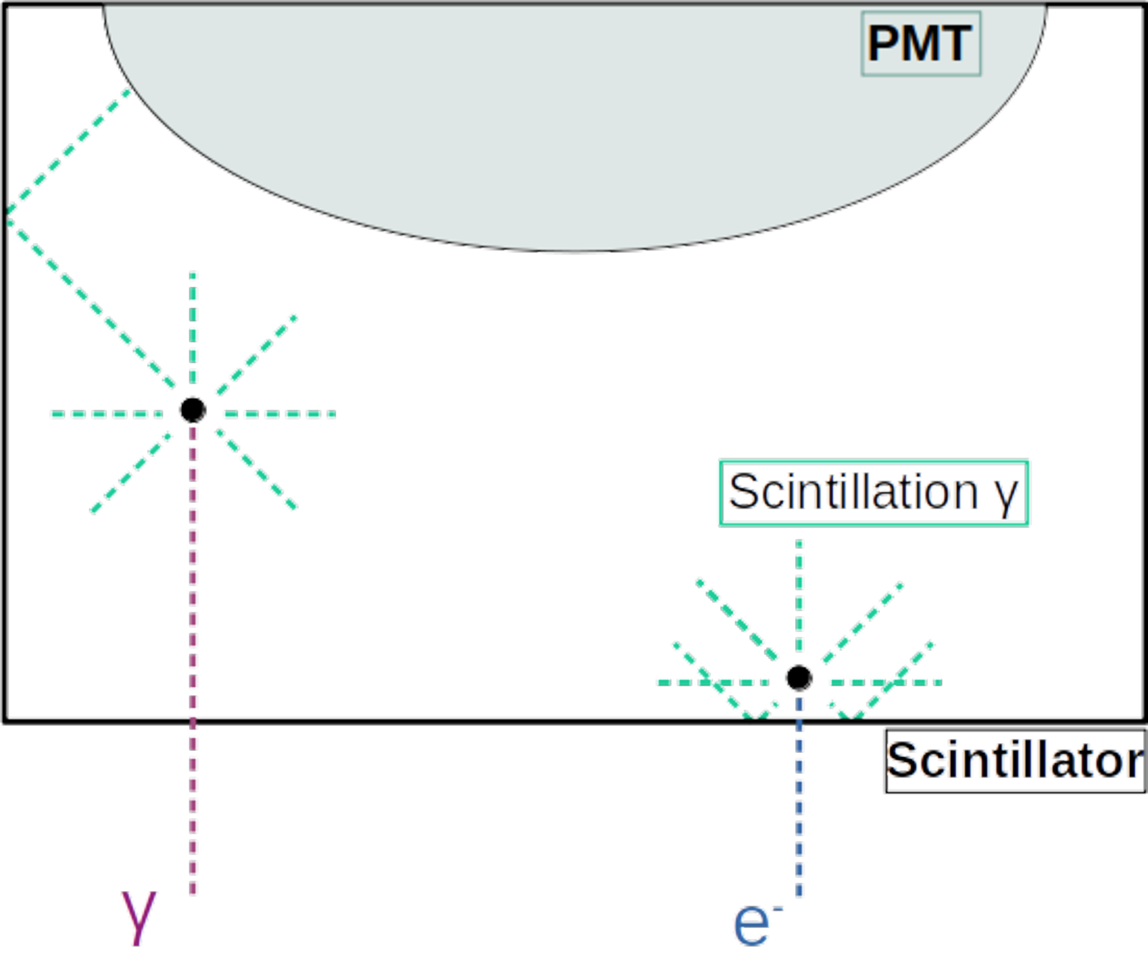
\includegraphics[width=8cm]{commissioning/fig_commissioning/Co_multi_reflection.pdf}
  \caption{A scheme of interaction of particles in a scintillator.
    The photon case is displayed on the left in rose dotted line, and the electron case is on the right in dark blue dotted line.
    Both particles enter in the scintillator through the front face.
    Examples of interaction points inside the scintillator are represented by the black dots.
    The photons of scintillation emitted after the interaction are materialised by the bright green dotted lines.
    Due to different interaction probabilities in matter, the two particles are stopped at different depths inside the calorimeter.
    The photon can interact deeply inside the volume of the scintillating material while the electron has a high probability to interact within the first few millimetres.
    \label{fig:photon_scintilator}}
\end{figure}
When the charged particle interacts in the scintillator, the absorbed energy leads to the emission of scintillation photons.
They propagate inside the scintillator, in all directions from the interaction point, at the speed $c/n_{sc}$, with $n_{sc}$ the optical index of the scintillator material and $c$ the speed of light in vacuum.
Depending on their initial direction, some of those photons propagate straightly to the PMT, and others are first reflected on the scintillator internal surface before entering the PMT, leading to time delay.

To illustrate this phenomenon and give an order of magnitude of this effect, we take the example of a photon interacting in the middle of the scintillator.
A photoelectron travelling straightly to the PM reaches the glass surface at $t_{s} = \frac{L}{2c/n_{sc}}$, $L$ being the scintillator width.
Now let consider a photoelectron emitted in the opposite direction.
It will propagate, reflect on the scintillator surface, and reach the PM at $t_{r} = \frac{3L}{2c/n_{sc}}$.
This photon is then delayed of $\Delta t = t_{r} - t_{s} = \frac{L}{c/n_{sc}}$.
Taking the width $L=25$ cm and $n_{sc}=1.5$, we obtain $1.25$ ns of delay.
Moreover, the more the incident particle interacts deeply inside the scintillator, the more those \emph{reflected photons} are delayed.
This mechanism increases the signal rising time collected at the PM anode, and impacts the scintillator time dispersion $\sigma_{t,\text{sc}}$.
In addition, giving the cross sections of particles in polystyrene, this effect is more important for incoming photons than for incoming electrons, for which it is quite negligible.
Therefore, we have $\sigma_{t,\text{sc}}^{\gamma}>\sigma_{t,\text{sc}}^{\text{e}^{-}}$.


\subsubsection*{Photomultiplier time dispersion}

The second term $\sigma_{t,\text{PM}}$ in Eq.~\eqref{eq:Co_sigma_t} describes the uncertainty on time measurement taken by the PM.
A photomultiplier is a photodetector: after the light is collected and converted on the photocathode, the photoelectrons are multiplied.
The time response depends on the transit time for the photoelectrons emitted at the photocathode to reach the anode after being multiplied.
This parameter influences only the absolute value of the time measurement and do not play a role in Eq.~\eqref{eq:Co_sigma_t}.
However, this transit time fluctuates for each photoelectron, this fluctuation being called the transit time spread (TTS).
It leads to an uncertainty on the time measurement and so has an influence on the photomultiplier time dispersion $\sigma_{t,\text{PM}}$.
\newline

In this study, we want to characterise the time dispersion bring by the photomultiplier on the time measurement.
To do so, we used a Cobalt $60$ source.

%% As displayed on Fig.~\ref{fig:supplied_voltage}, these characteristic times depend essentially on the supplied voltage.
%% \begin{figure}[h]
%%   \centering
%%   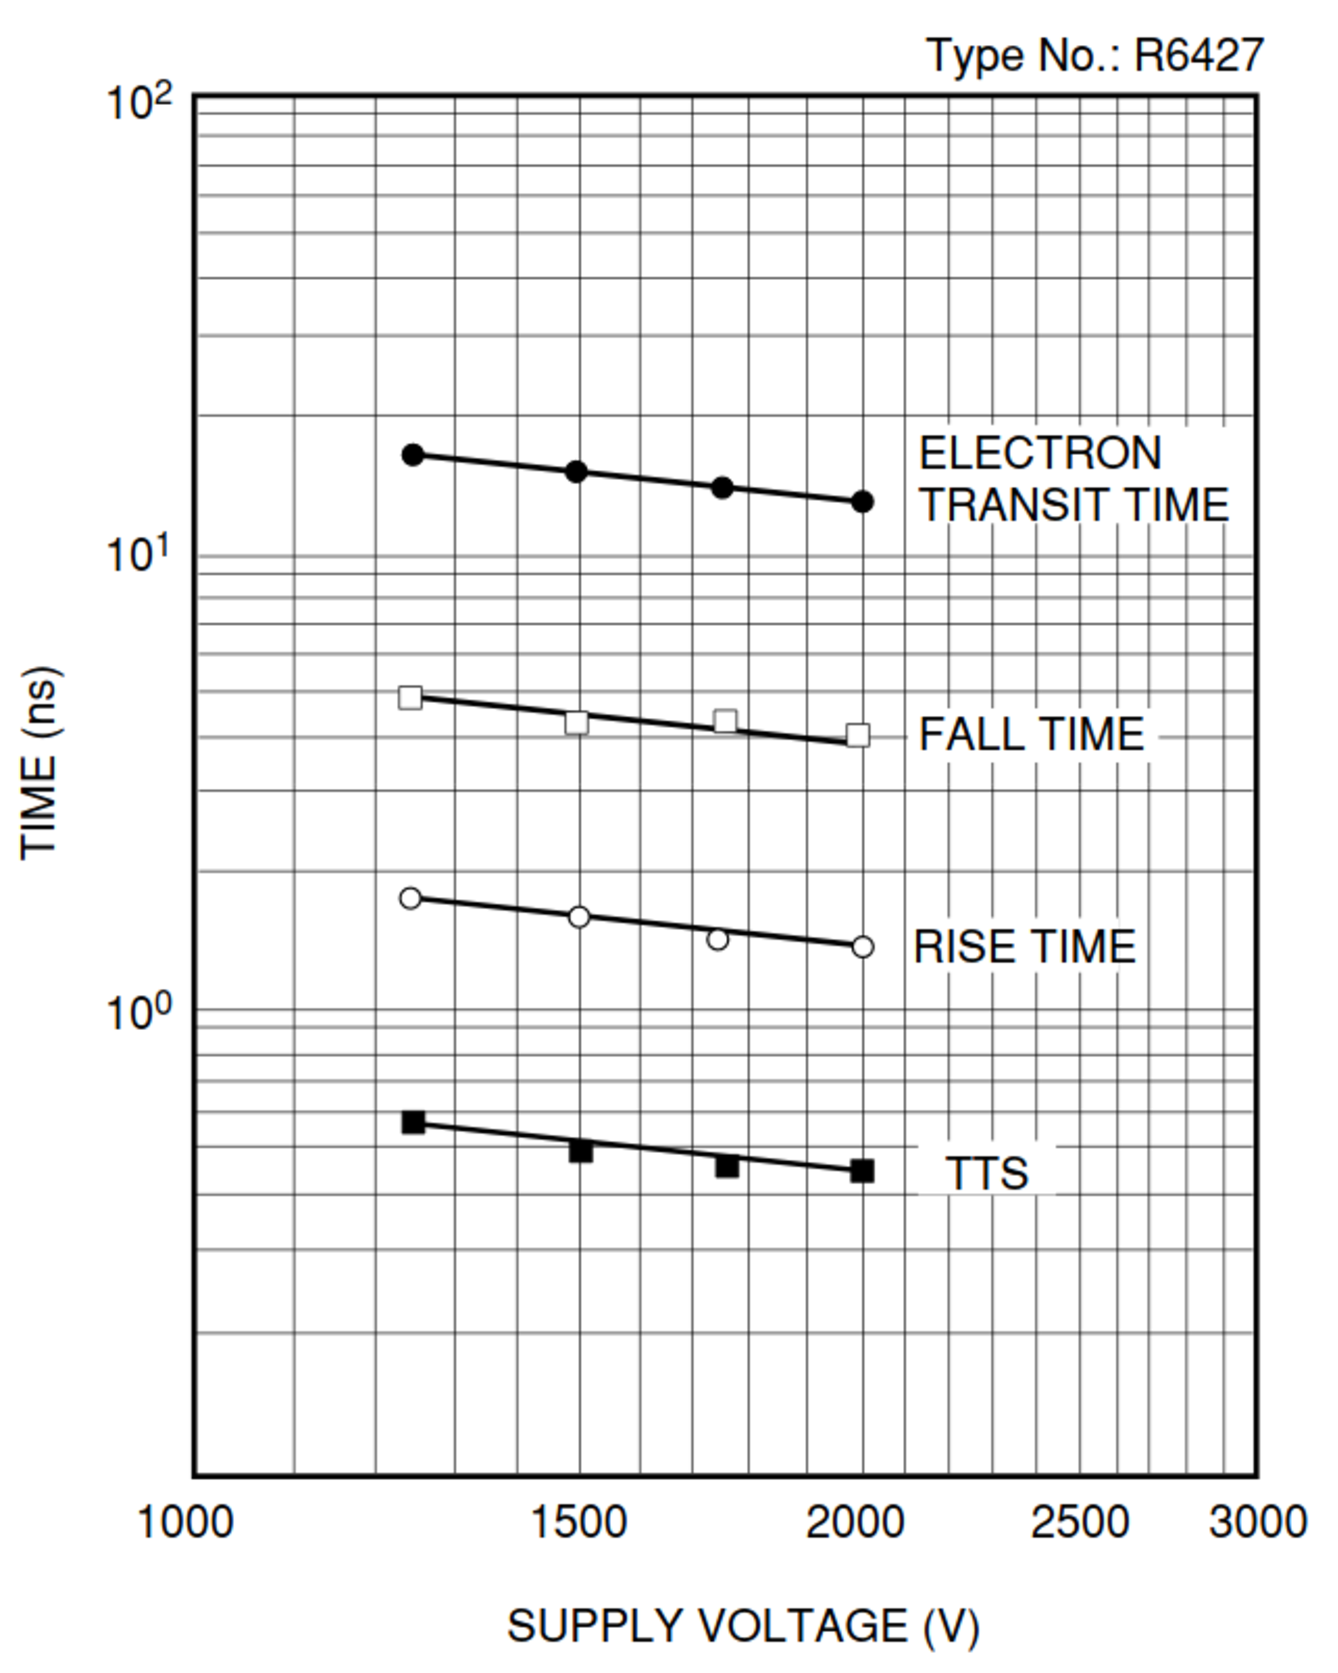
\includegraphics[width=8cm]{commissioning/fig_commissioning/PM_supplied_voltage.pdf}
%%   \caption{Different characteristic times of a photomultiplier (R$6427$) with the supplied voltage.
%%     The electron transit time, falling time, rising time and time transit spread (TTS) are displayed.
%%     The higher the supplied voltage, the better the characteristic times.
%%     \label{fig:supplied_voltage}}
%% \end{figure}

%% 231.8e3  1s
%% 1e9
%% 71.9 minutes equiv. temps run pour simus
%% normalisation simus : Nev * 0.375

\subsection{Energy calibration of optical modules}
\label{subsec:OMenergyCalib}

As described in Sec.~\ref{sec:OMtimeResponse}, the collected charge at PM voltage divider is proportional to the amount of incident photoelectrons, and then to the initially deposited energy inside the scintillator.
Once optical modules were assembled (optical coupling, packing, shielding integration), they were individually tested at Bordeaux laboratory, CENBG.
Their energy resolutions for $1$ MeV-electrons at the centre of scintillator front face were determided.
High voltages were set to optimal values, aligning their gain at $300$ mV at $1$ MeV.
However, after calorimeter integration, du to different environement, amplitude spectra of each optical block have to be re-aligned.
This work was performed by Axel Pin, PhD student at CENBG.
We give in this section a summary of this energy calibration study.



\subsection{Experimental setup}

Cobalt $60$ is an man-made isotope with a half-life of $5.27$ years.
The initial activity of the source we used to achieve this setup was $447.4$ kBq in $2014$.
This activity was reduced to $232$ kBq at the time of the data taking.

The main goal of this study is to provide a time calibration for all optical modules of both main walls.
%% precise XW GV
As the demonstrator is closed at this time, placing the source in the middle of the detector is not possible.
The better solution is to put it behind the main walls.
In order to be sure all PMs receive light from the source, we decide to place it at $9$ different positions per wall, approximatively one meter behind the PMs.
We take $18$ runs roughly $20$ minutes long.


\begin{figure}[h]
  \centering
  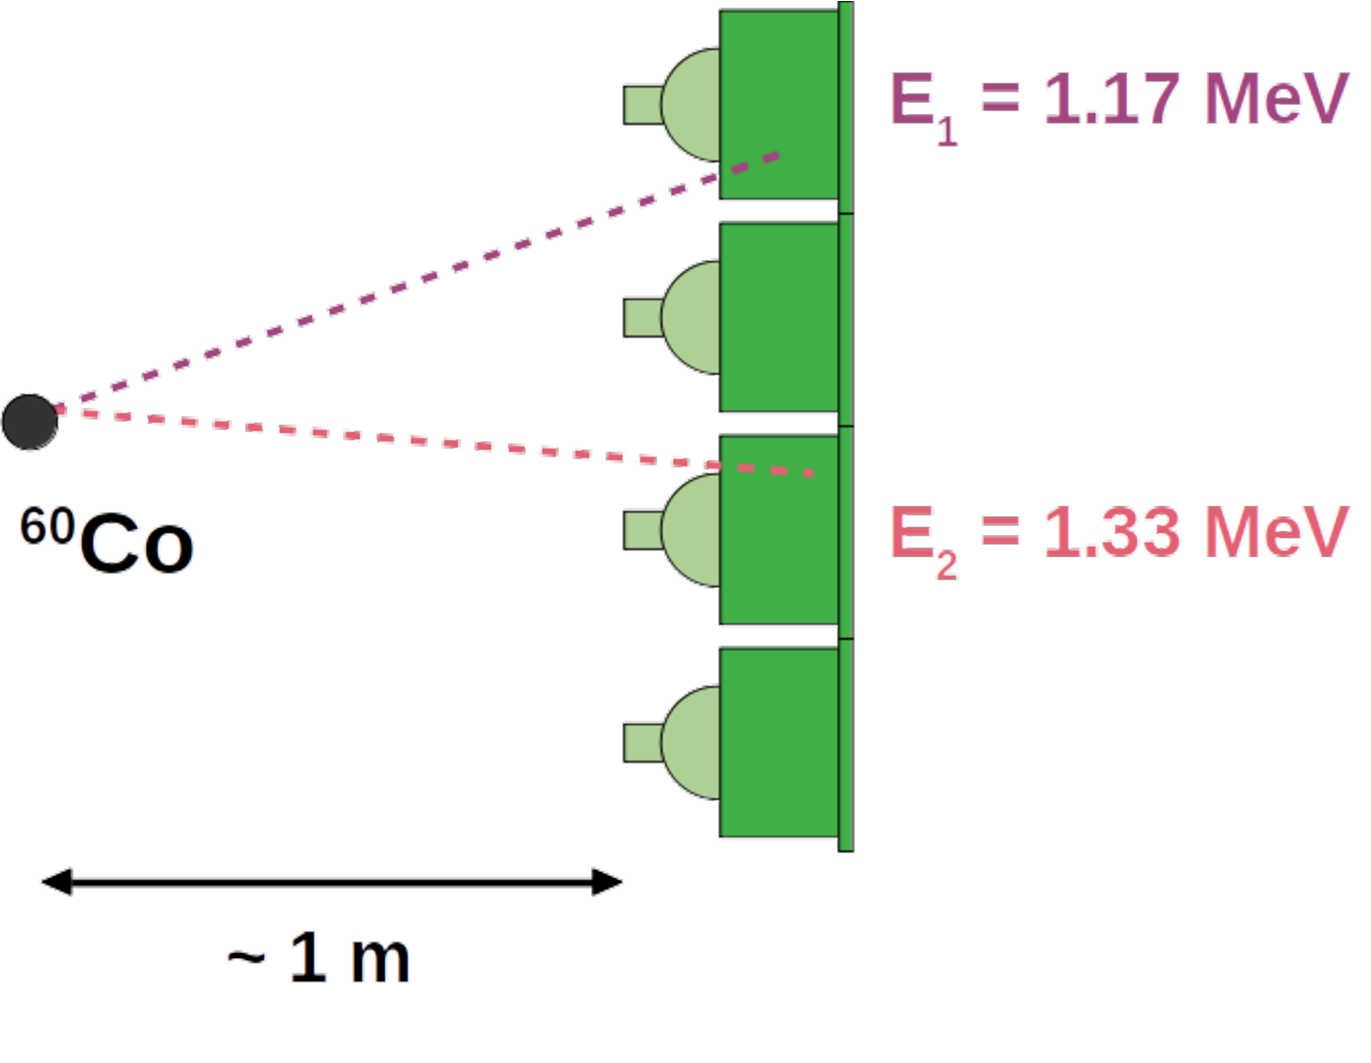
\includegraphics[width=6cm]{commissioning/fig_commissioning/Co_setup.pdf}
  \caption{
\label{fig:}}
\end{figure}

\subsection{Detector efficiency}
\label{subsec:detector_efficiency}

As decsribed in Sec.~\ref{sec:SNsoftware} of chapter~\ref{ch:detector}, the SuperNEMO collaboration developed its own simulation, reconstruction and analysis environement.
The Falaise software, specifically designed by and for the SuperNEMO collaboration, holds the \verb!C++! library for the event reconstruction and analysis of simulated and real data.
Especially, it contains the geometry, the detector material, the event data model, the reconstruction algorithms and the data analysis.
Finally, the SNFee software is a tool package for the parametrisation, control and monitoring of the SuperNEMO front-end electronics.
All this software environement has been used in the framework of the current Cobalt analysis.

In order to monitor and compare the real data, I performed \Co\ event simulations in the SuperNEMO demonstrator, using the Falaise software.
To match the real data, the simulated source has been placed behind one of the two calorimeter main walls of the detector.
In fact, at this time, the simulated detector is symetrical in terms of detection perfomances.
Therefore, simulations of \Co\ events behind the two main walls are equivalent.
Consequently, we only simulated the \Co\ source behind the Italian main wall, and used these simulations for both main calorimeter walls.
The Falaise and Root softwares have been employed to analyse the simulated data.

As we said, the main goal of this study is to use the \Co\ decay to calibrate in time the optical modules.
Then, the signal we are looking for is the detection of the $2$ photons of $1.17$ MeV and $1.33$ MeV we described above.
To maximise the ratio signal over background, some cuts have been applied on the real and simulated data.
\begin{itemize}
\item Coincidence time criterion:\\ we define the coincidence time window by events occurring in a $62.5$ ns-long time interval.
  This allows to avoid accidental coincidence events.
\item Trigger criteria:\\ we are interested in events that passed both the low and high thresholds, corresponding to $150$ keV and $300$ keV, respectively.
  Moreover, we only keep events with exactly two triggering electronic channels in the selected coincidence time window and for the given trigger conditions.
\item Individual energy cuts:\\ given the two photon energies, we only select individual calorimeter hit energies greater than $0.7$ MeV.
\end{itemize}
In Fig.~\ref{fig:detector_efficiency}, we compare the real and simulated energy spectra for \Co\ events satisfying to the three criteria described above.
\begin{figure}[h]
  \centering
  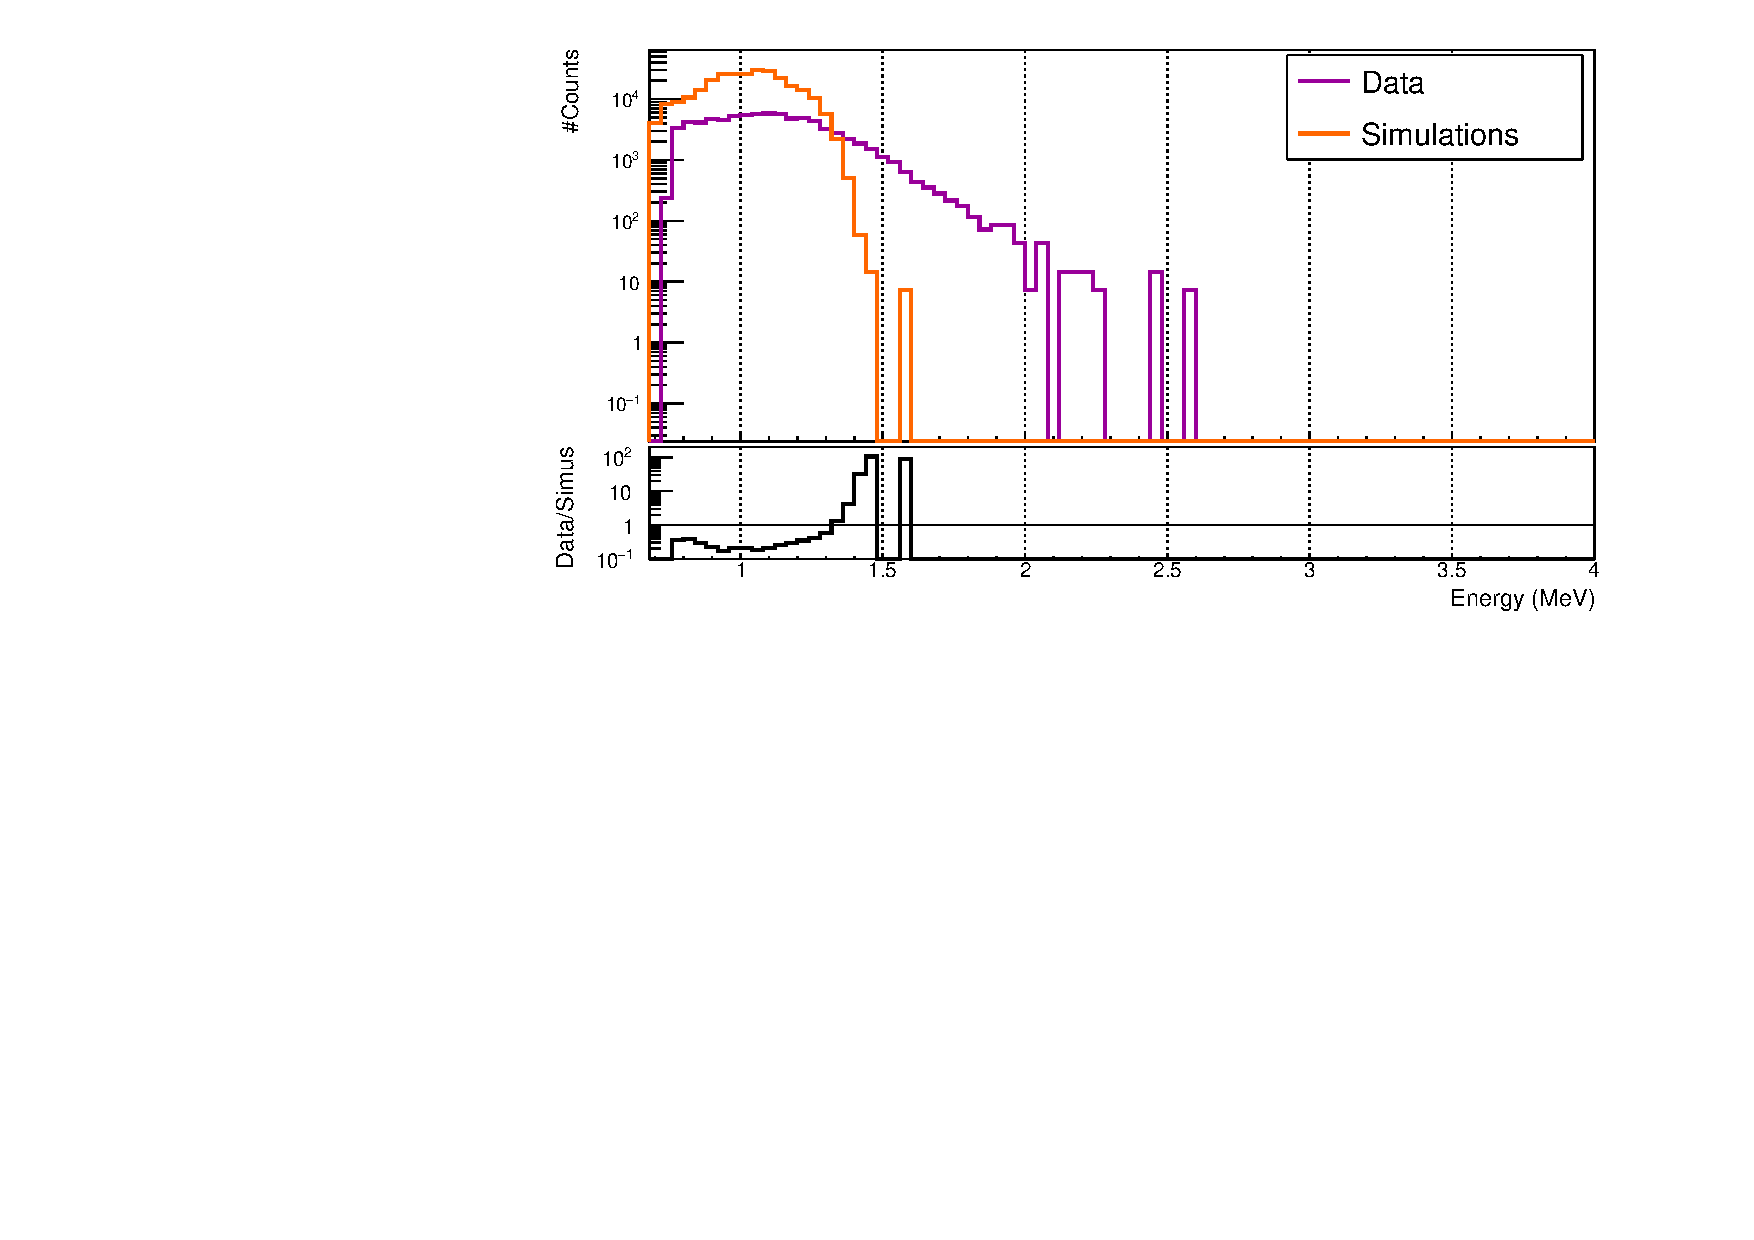
\includegraphics[width=17cm]{commissioning/fig_commissioning/Co_efficiency_detector.pdf}
  \caption{Top pad: energy spectra for simulated data (orange plain line) and real data (purple plain line) in logarithmic scale.
    Bottom pad: ratio of real data over simulated data for each bin in logarithmic scale.
\label{fig:detector_efficiency}}
\end{figure}
The simulated data are normalised to the source activity and the run time.
We notice the Compton edge of the \emph{first} $1.17$ photon
\footnote{Looking at Fig~\ref{fig:Co_decay_scheme}, the first photon to be emitted after the Cobalt $\beta$ decay is the one at $1.17$ MeV.
  Then, we name it \emph{first} photon, the one of $1.33$ MeV being called the \emph{second} photon.}
is at $0.96$ MeV, and the one of the second photon at $1.11$ MeV.
Therefore, given the energy resolution of optical modules, the Compton edge of the second photon is located in the energy peak of the first photon.
On the simulated energy spectrum, we observe three different energy peaks.
The first one, located around $0.95$ MeV, is the Compton edge of the $1.17$ MeV energy photon.
The second peak stands around $1.1$ MeV. It is a mixing between the energy of first photon, and second photon Compton edge.
Finally, the third energy peak, around $1.3$ MeV, represents the detection of the second photon.

We immediately notice the different shape of real data energy spectrum.
Firstly, we do not distinguish the three energy peaks.
This may be caused by several reasons.
Firstly, the energy resolution of the calorimeter blocks.
Secondly, at the time of the data taking, optical modules where not equalised in gain.
Secondly, the real data energy spectrum is characterised by a high energy part.
This may be due to background, which are not taken into account in the simulated data.
In the following is presented a background analysis to investigate the high energy part of the energy spectrum, and better understand the data.

Given the amount of real and simulated events, we conclude that the detection efficiency is $29$\%.
Numerous parameters can affect the detection efficiency.
\begin{itemize}
\item Read out efficiency is mainly driven by
\end{itemize}



Efficiency is going to be improuved.

\subsection{Background estimation}

At the time of data taking, the calorimeter of SuperNEMO was in commissioning phase, with some implications for the current analysis.
Firstly, the external shielding was not yet installed, so the calorimeter was not protected from background coming from laboratory.
Secondly, the energy calibration discussed in Sec.~\ref{subsec:OMenergyCalib} was not completed, and optical modules' gains were not all aligned.
These two statements may impact this study's results.

In this section, we want to estimate the amount of background events for each optical module for the data taking time period.
The main background type are $\gamma$'s emitted during disintegration of \Tl\ and \Bi\ isotopes, coming from natural radioactivity ($^{238}$U and $^{232}$Th decay chains respectively).

Unfortunately, we do not have a background run for this time period.
However, we can extract informations on background events from data runs taken with the Cobalt source placed behind the wall.
We suppose the more one optical block is far from the source, the more the ratio signal over background decreases.
The idea here is to look only at the data taken with the part of optical modules \emph{far} from the source.


To estimate the number of background event received by each optical module by unit of time, we have to estimate the signal over background ratio for optical modules far from the Cobalt source.
To do so, we pick a run for which the Cobalt source is far from most of the optical modules of the wall, that is to say, placed at a main wall corner.
We then select events occuring far from the source.
We want to check if this approximation is correct.

plot hit energy/distance with source?

\emph{idea : regarder la stat/forme du spectre en fonction de la coupure}


\subsection{Determination of the individual timing resolution of each optical module}

Optical modules have been characterised before installation.
Performing simulations of \Co\ disintegration

The final goal of this analysis is to determine the time resoltion of optical modules, due to the scintillator time dispersion.
As displayed in Fig.~\ref{fig:Co_decay_scheme}, the two photon of Cobalt $60$ are emitted in coincidence.
The cuts described in Sec.~\ref{subsec:detector_efficiency} aim to maximise the ratio signal over background, the signal being the detection of two $\gamma$s interacting in two different optical modules.
The two $\gamma$s, travelling at speed of light in air, reach the two optical modules at two different times.
The arrival time of a particle in a given optical block $t^{\gamma}_{i}$, descibed in Fig.~\ref{fig:CFD} in Chapter~\ref{ch:commissioning}, is defined from the amount of charge collected at PM anode and received by the electronic readout.
We are interested in event topologies where the two $\gamma$s of Cobalt $60$ hit two different calorimeter blocks.
We then look for topologies where two calorimeter hits occured in a given time window of $60$ ns.
This coincidence time window where chosen to select the two Cobalt $\gamma$s coincidence events, avoiding accidentals.
Taking two distinct optical modules $A$ and $B$, we define the time difference between the two calorimeter hits as $\Delta t = t^{\gamma}_{A} - t^{\gamma}_{B}$.
In Fig.~\ref{fig:Co_deltat} is presented an example of $\Delta t$ distribution for two optical modules.
\begin{figure}[h]
  \centering
  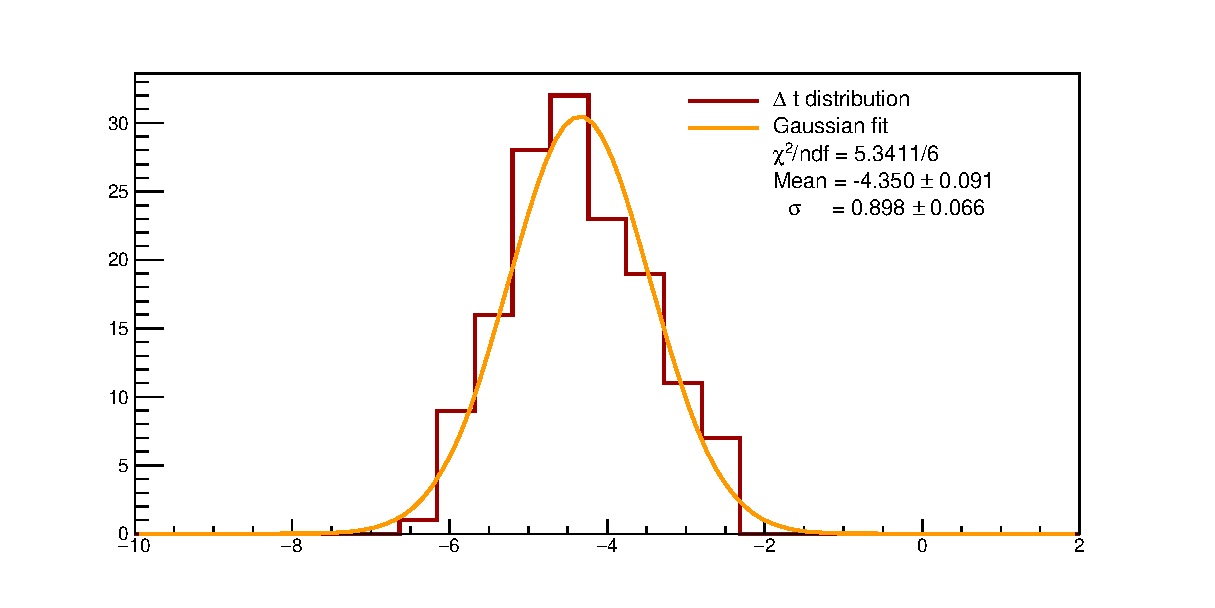
\includegraphics[width=15cm]{commissioning/fig_commissioning/Co_deltat_distrib_ex.eps}
  \caption{\label{fig:Co_deltat}}
\end{figure}
Each optical module pair is then characterised by the mean and the $\sigma$ of this distribution, whose depend mainly on three parameters:
\begin{itemize}
\item the distance from the Cobalt source to the wall,
\item the distance between the two optical modules condidered,
\item the time made by the electric signal to travel from a PM divider to the electronic readout.
  In other words, the time difference distribution for a given pair of optical module is affected by the difference of lengths of the two coaxial cables from the PMs divider to the electronic channel.
\end{itemize}
For two given optical modules,


%%%%%%%%%%%%%%%%%%%%%%%%%%%%%%%%%%%%%%%%%%%%%%%%%%%%%%%%%%%%%%%%%%%%%%%%%%%%%%%%%%%%%%%%%%%%%%%%%%%%%%%%%%%%%%%%%%%%%%%%%%%%%%%%
\section{The Light Injection System}
\label{sec:LIS}

The SuperNEMO demonstrator is designed to have a long exposure time.
In this context, calibration systems are necessary to control and calibrate the response of the detector.
The so called \emph{Light Injection} (LI) System will monitor the stability of the calorimeter response in energy to $1$\%.
It consists in $20$ Light Emitting Diodes (LED) at $385$ nm, injecting light in each scintillator block via optical fibers.
A set of reference optical modules (PMTs coupled with scintillator blocks), receiving light from both LEDs and $^{241}$Am sources, monitors the stability of the LEDs.
A scheme of the complete LI calibration system is given in Fig.~\ref{fig:LIS_scheme}.

First LI commissioning data was taken in March 2019.



\begin{figure}[h]
  \centering
  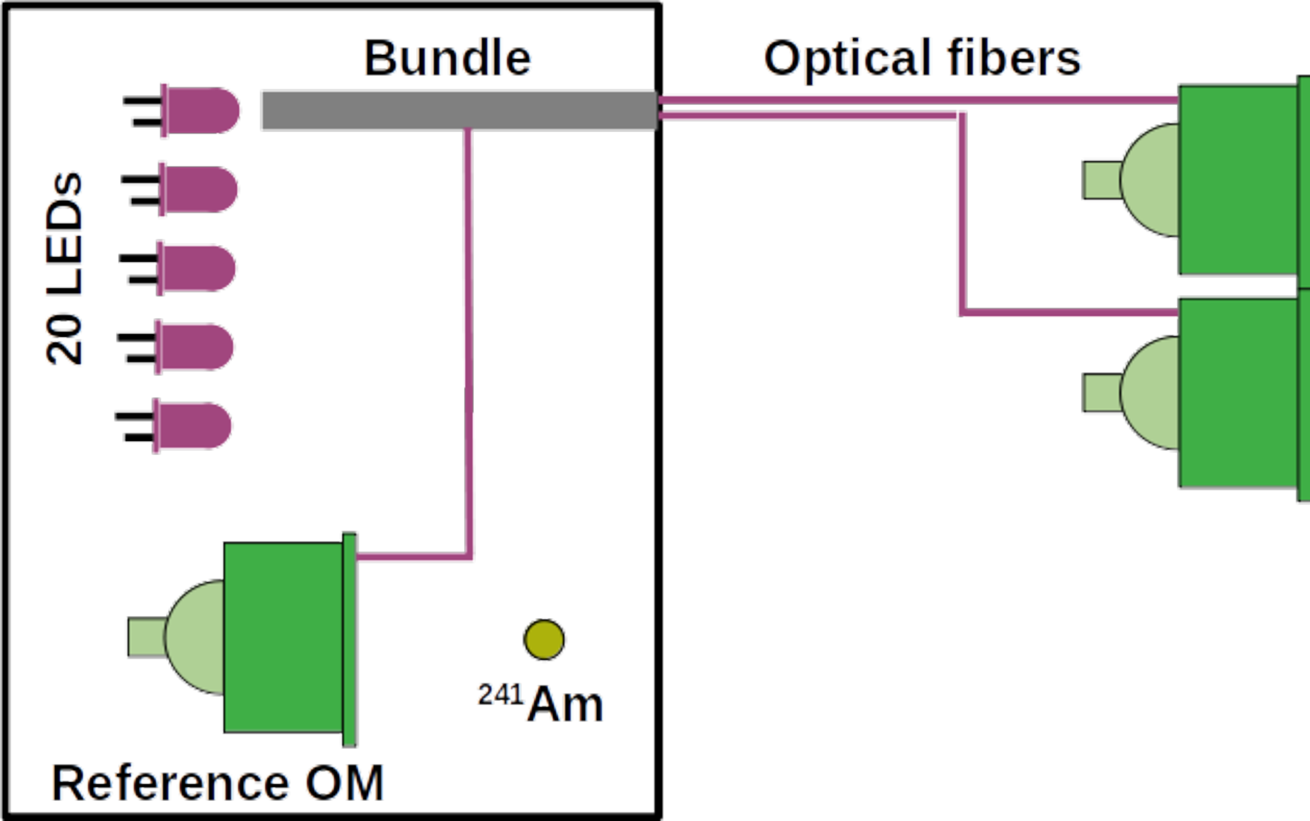
\includegraphics[width=10cm]{commissioning/fig_commissioning/LIS_scheme.pdf}
  \caption{The Light Infection (LI) calibration system is schematised.
    More than $1300$ fibers, distributed in $20$ bundles, carry the light from $20$ LEDs to each scintillator block of the demonstrator.
    Reference OMs coupled with $^{241}$Am sources monitor the LED light.
    \label{fig:LIS_scheme}}
\end{figure}

\subsection{Light injection system commissioning}


In the LI system design, the SuperNEMO demonstrator has been segmented in $10$ areas.
Each area receives light from one given LED

Primary/secondary
Each LED lights
Group LEDs/area

\begin{figure}[h]
  \centering
  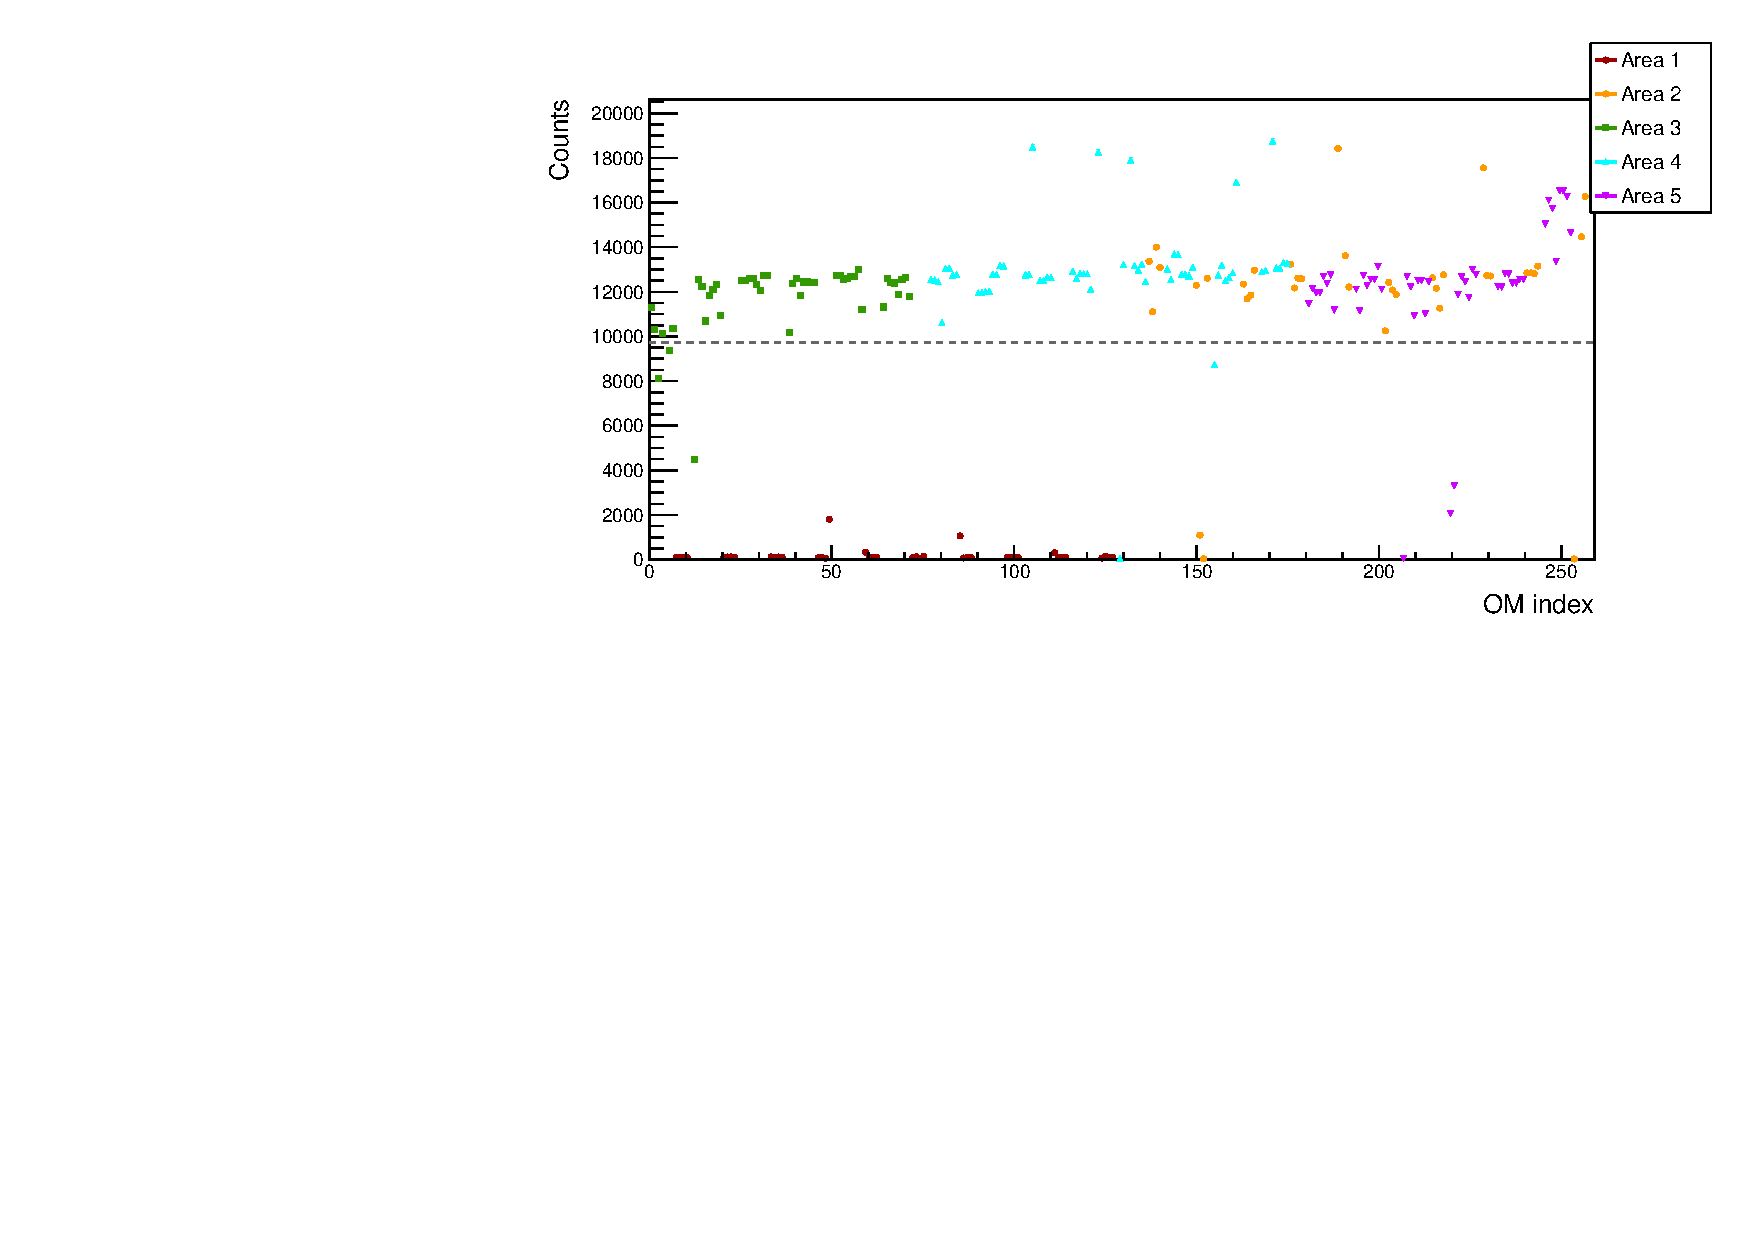
\includegraphics[width=15cm]{commissioning/fig_commissioning/LI_1d_counts.pdf}
  \caption{The number of counts is displayed for each optical module, labelled by the \emph{OM index}.
    Each coloured marker represents counting rates for one area of the detector, that is to say one group of optical modules lighted by the same LED.
    The area \#$1$ (dark red dots) is not receiving light from its corresponding LED.
    \label{fig:LI_counts}}
\end{figure}


\begin{figure}[h]
  \centering
  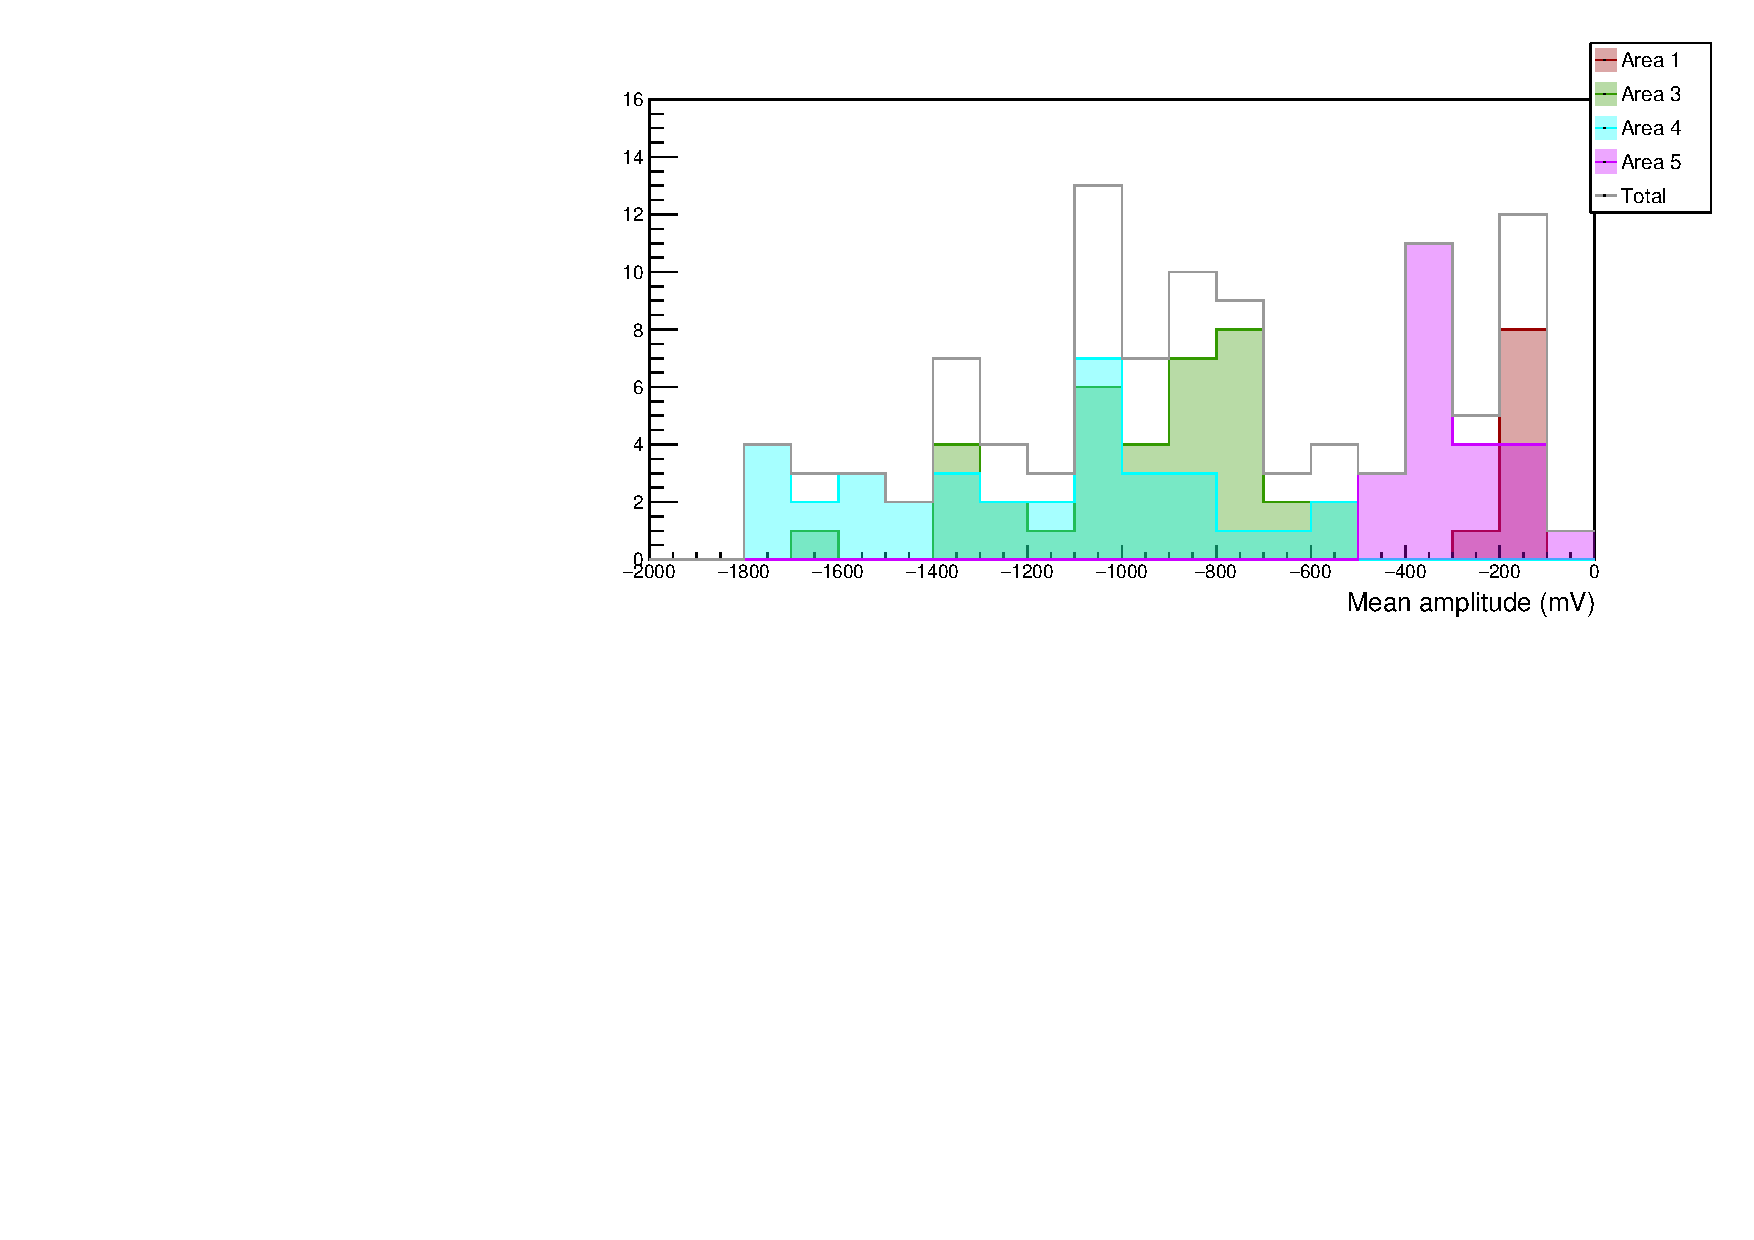
\includegraphics[width=15cm]{commissioning/fig_commissioning/LI_mean_ampl.pdf}
  \caption{The mean signal amplitude distribution for each optical module is presented.
    One colour stands for one area of the half detector.
    In Grey is the total mean amplitude distribution.
    \label{fig:LI_ampl}}
\end{figure}


\subsection{Time resolution of optical modules}



%% \begin{figure}[h]
%%   \centering
%%   \includegraphics[width=10cm]{commissioning/fig_commissioning/}
%%   \caption{
%% \label{fig:}}
%% \end{figure}



%% \begin{figure}[h]
%% \centering
%% \begin{subfigure}[t]{0.48\textwidth}
%%   \centering
%%   \includegraphics[width=1.1\textwidth]{commissioning/fig_commissioning/}
%%   \captionsetup{justification=centering}
%%   \caption{
%%     \label{subfig:}}
%% \end{subfigure}
%% \hfill
%% \begin{subfigure}[t]{0.48\textwidth}
%%   \centering
%%   \includegraphics[width=1.1\textwidth]{commissioning/fig_commissioning/}
%%   \captionsetup{justification=centering}
%%   \caption{
%%     \label{subfig:}}
%% \end{subfigure}
%% \caption{
%%   \label{fig:}}
%% \end{figure}
